\documentclass[a4paper, 11pt]{book}
\usepackage[utf8]{inputenc}
\usepackage{minted}
\usepackage{graphicx}
\usepackage{hyperref}
\usepackage[linguistics]{forest}
\usepackage{bussproofs}
\usepackage{wrapfig}
\usepackage{xspace}
\usepackage{xpatch}
\usepackage[firstpageonly=false]{draftwatermark}
\usepackage{amsfonts}
\usepackage{amssymb}
\usepackage{mathbbol}
\usepackage{stackengine}

\SetWatermarkText{Draft \today}

\SetWatermarkScale{.7}
\SetWatermarkAngle{30}
\SetWatermarkColor{red!50!white}

\SetWatermarkHorCenter{0.15\paperwidth}
\SetWatermarkVerCenter{0.08\paperheight}


\makeatletter
\AtBeginEnvironment{minted}{\dontdofcolorbox}
\def\dontdofcolorbox{\renewcommand\fcolorbox[4][]{##4}}
\xpatchcmd{\inputminted}{\minted@fvset}{\minted@fvset\dontdofcolorbox}{}{}
\makeatother

\newenvironment{bprooftree}
  {\leavevmode\hbox\bgroup}
  {\DisplayProof\egroup}
  
\hypersetup{
    colorlinks,
    linkcolor={red!50!black},
    citecolor={blue!50!black},
    urlcolor={blue!80!black}
}
\usepackage[backend=biber,style=alphabetic]{biblatex}
\DeclareUnicodeCharacter{2200}{$\forall$}
\DeclareUnicodeCharacter{03BB}{$\lambda$}
\addbibresource{hdr.bib}
\addbibresource{other.bib}

\DeclareSourcemap{
  \maps[datatype=bibtex, overwrite]{
    \map{
      \perdatasource{hdr.bib}
      \step[fieldset=keywords, fieldvalue={, }, appendstrict]
      \step[fieldset=keywords, fieldvalue=me, append]
    }
    \map{
      \perdatasource{other.bib}
      \step[fieldset=keywords, fieldvalue={, }, appendstrict]
      \step[fieldset=keywords, fieldvalue=they, append]
    }
  }
}
%'theorem.py:CoqLexer -x'
\newminted[elpicode]{elpi.py:ElpiLexer}{fontsize=\small,autogobble,escapeinside=~~,mathescape=true,frame=leftline,framerule=0pt,framesep=1em}
\newminted[elpicodelj]{elpi.py:ElpiLexer}{fontsize=\small,autogobble,escapeinside=~~,mathescape=true,frame=leftline,framerule=0pt,framesep=0em}
\newmintinline[elpi]{elpi.py:ElpiLexer}{fontsize=\small,autogobble,escapeinside=~~,mathescape=true,frame=leftline,framerule=0pt,framesep=1em}
\newminted[rocqcode]{theorem.py:XCoqLexer}{fontsize=\small,autogobble,escapeinside=~~,mathescape=true,frame=leftline,framerule=0pt,framesep=1em}
\newmintinline[rocq]{theorem.py:XCoqLexer}{fontsize=\small,autogobble,escapeinside=~~,mathescape=true,frame=leftline,framerule=0pt,framesep=1em}
 
\newminted[ocamlcode]{ml.py:OcamlLexer}{fontsize=\small,autogobble,escapeinside=~~,mathescape=true,frame=leftline,framerule=0pt,framesep=1em}
\newmintinline[ocaml]{ocaml}{fontsize=\small,autogobble,escapeinside=~~,mathescape=true,frame=leftline,framerule=0pt,framesep=1em}

\newenvironment{dedication}
  {%\clearpage           % we want a new page          %% I commented this
   \thispagestyle{empty}% no header and footer
   \vspace*{\stretch{1}}% some space at the top
   \itshape             % the text is in italics
   \raggedleft          % flush to the right margin
  }
  {\par % end the paragraph
   \vspace{\stretch{3}} % space at bottom is three times that at the top
   \clearpage           % finish off the page
  }
\title{Elpi: rule-based extension language}
\begin{document}
\maketitle
\chapter*{Dedication}
\begin{dedication}
To Cinzia and Anna
\end{dedication}

\setcounter{tocdepth}{5}
\tableofcontents

 \chapter{Introduction}


\section{Prologue}

\subsection{Beyond the odd order theorem}

I had the luck to be part of this project.
After its completion the good question was what it made it possible
other than having Georges Gonthier lead the project. How to make
it possible for others to build such an impressive machine checked
proof. I've always been interested into building tools, since I believe
a tool can democratize...

3 points 1) engineering practices, not new but too often
ignored by the community; 2) formalization technique known as boolean
reflection (or small scale reflection) that carves a light weight
``classical math'' framework in Rocq (EM, UIP, FUNEXT) in Rocq when
constructivism allows for it; 3) ``creative'' programming of the
Rocq elaborator.

We focused on 3. These programs make Rocq behave as an informed readers,
that is a reader that knows some base facts and that is expected to
be able to combine them using some well known rules. It was customary,
at that time, to see Rocq as a ``dumb reader'': you have to explain
every single detail to him. These programs changed the game  for the
oothm and made it possible to use notations as in math, that is convoy
a lot of information implicitly, by convention.

The objective was to help users craft these programs. Programming
the elaborator as we did was hard. Structuring the library to that
knowledge could be organized by the author an retrieved by these
programs was even harder. The programming mechanism is called CS,
and is strictly related to the UH I studied during my PhD.
Independently, about at the same time,
Rocq got extended with type classes, which happened to be usd for similar
purposes, and immediately raised similar programming issues.

To my eyes, these programs were strikingly related to Prolog.
Our programs were organized in rules and driven by unification.
At that time I had barely heard about Prolog.
It happened that the Parsifal team
at Inria Saclay worked on a language or that family
and thanks to Assia Mahboubi and Stephane Legrand I could give a talk
at a STTT workshop they were hosting.

In my talk I did explain some of the programs we wrote and why they
were helping us writing math in Rocq. Dale Miller, asked a few questions
and suggested that his $\lambda$Prolog language was probably what I
was looking for, but since I did not know anything about it I could
just nod and ask to continue to the discussion offline.

not just the rules but also their animation and maybe also the entire
elab algorithm.

Dale was kind
to set up a meeting with Claudio Sacerdoti and myself. 

\subsection{The beginning: a snowy day}

On that day ``Paris'' was frozen, in the sense that a supposedly
``show storm'' convinced authorities to close buildings and other facilities,
reduce public transportations to the bare minimum. For some reasons
the XXX building was not closed, so the 3 of us agreed to buy a sandwich,
walk up the hill (with boots) and meet in a desert building.

After two hours of gentle introduction, after having savoured the
elegance of \elpi{copy}, I clearly remember I say ``sold...'',
but I also completed the sentence with ``how do I do evars?''.

$\lambda$Prolog could easily describe the rules my programs were
made of and elegantly manipulate the data type of Rocq terms that
notably contains many binders. But also holes, evars in Rocq slang,
that are the other beast one has to tame in order to implement an
elaborator and, in general, the outern layers of a toll like Rocq.

It was the beginning.

Teyjus in bologna, we could write a toy elaborator in one day
but we could not find a good solution. Reification is ugly, one has
to pass a subst and reimplement unif. At the same time reusing unif
variables seemed possible, but extremely hard since the pure core
of LP, and Teyjus, do not really give you systems to control their
assignment and an elaborator takes in input a term with holes
and returns a term where only some holes are assigned...

It was worth trying but using teyjus in Matita or Rocq was too hard.
I write a POC interpreter of LP in OCaml for embedding it into
Matita and Rocq, elpi. It was easy to add hacks and experiment with
it, and that ... Elab in matita was kind of working, we could run
it on the arithmetic library. It was clear that:
the perf were bad, very bad, like 22K times bad.
the hacks could be explained in terms of constraints and rules to
suspend, resume, combined them.


\section{Elpi}
Elpi is both a language and an implementation of that language.

With CSC we rewrote the runtime, first the FO part then the HO part
and 

line stats

I perceived many times, in academic circles, some mistrust in logic programming.


We organize this document in four parts. The first two describe Elpi from
A to Z, both as a language and as an implementation of that language (we credit
\cite{ridoux1998lambda}). The third describes the integration of Elpi in Rocq
and the fourth one surveys the application developed for Rocq using Elpi.


\chapter{Elpi the language: \emph{de A \`a Z}}

Elpi is a mix of two languages: $\lambda$Prolog and Contraint Handling Rules.
The former is a higher order variant of Prolog based on
Hereditary Harrop Formulas, a generalization of Horn Clauses.
The latter is language to manipulate a store of constraints that,
in the case of Elpi, is made of suspended goals, i.e. sequents
made of heigenvariables, dynamic rules and a conjecture.

We briefly introduce all the ingredients that constitute Elpi.
Most of the syntax of Elpi is inherited from $\lambda$Prolog, as well
as the type discipline~\cite{Miller_Nadathur_2012}; similarly most of
its dynamic semantics is inherited from Prolog.
We state this upfront with no claim of novelty but we will just say Elpi in what
follows. We shall still highlight the novelties or simply differences from
$\lambda$Prolog or Prolog as they appear.

\section{Elpi v.s. Prolog}

Regarding an introduction to Prolog, the reader is spoiled for choice.
Here, we limit ourselves to establishing the terminology and highlighting
the key characteristics of Elpi and differences from standard Prolog from the
perspective of the programmer. We identify three of them: data types, rules
and search.

The first feature worth pointing out is algebraic data types, such as
list and trees. Here the declaration of binary tress in Elpi syntax:

\begin{elpicode}
kind tree type.
type leaf tree.
type node int -> tree -> tree -> tree. 
\end{elpicode}

The \elpi{leaf} and \elpi{node} symbols can be used to
build terms and have arity 0 and 3 respectively. Elpi
follows the tradition of typed functional languages by prescribing not only
an arity but a more precise type to \elpi{leaf} and \elpi{node}.
In this document we refer to them as term constructors, or simply constructors.
\begin{wrapfigure}{r}{.2\textwidth}
  \begin{forest}
    [46 [93 [-] [-]] [-]]
  \end{forest}
\end{wrapfigure}
Types play no role at run time but grately contribute to the static analysis
of the code, allowing to report typos and sometime even true errors, early.
As an example the term
\elpi{(tree 46 (tree 93 leaf leaf) leaf)}
represents the tree depicted on the right.
To the reader familiar with
Prolog we point out that Elpi adopts the syntactic convention
of $\lambda$-calculus for function calls, namely $(f~ x~ y)$ rather than the
mathematical convention $f(x,y)$ adopted by Prolog.


The second feature we discuss is that the code is organized into
rules, that constitue the smallest code unit\footnote{In this document we prefer the
word rule to clause.}. A rule is made of two parts, the head and the premises.
Intuitively the head drives the selection of a rule, reducing the current
problem, that we goal, to simpler ones. Operationally the head is unified with the
goal, possibly assigning value to the rule parameters that are embodied by
unification variables. As an example we provide the code computing the size of
a tree, together with its signature:

\begin{elpicode}
type size tree -> int -> prop.
size leaf 0.
size (node _ L R) N :- size L N1, size R N2, N is 1 + N1 + N2.
\end{elpicode}
Again we favor a type assignment to a simple arity. \elpi{prop} is the
type of executable code, meaning that \elpi{size}, when applied to two
arguments, becomes a goal and a program can be run to solve it.
On the contrary \elpi{node}, applied to any number of arguments,
is just a piece of data, it is not a goal.

\begin{elpicode}
goal> size T N.

Success
  N = 2
\end{elpicode}
Operations on built-in data types, such as integers, are provided via
the built-in \elpi{is} operator that evaluates its right hand side
and unifies the result with the left hand side.
~\\
It is worth pointing out that variables do not need to be used linearly
in the head of a rule: since the head is unified with the goal, it makes sense to
write there any therm, not just terms that happen to be patterns in
the sense of functional programming languages. For example the following
piece of code succeeds only if the tree is empty or made of two
identical subtrees.

\begin{elpicode}
type symmetric tree -> prop.
symmetric leaf.
symmetric (node _ T T).
\end{elpicode}

The third characteristic is that Elpi internalizes a form of search called
backtracking: all rules are potentially applied and there is no committment to
the first rule whose head unifies with the goal.
Here an example of code relying on backtracking to test
the membership of an element ot a tree.

\begin{elpicode}
type mem tree -> int -> prop.
mem (node N _ _) N.
mem (node _ L _) N :- mem L N.
mem (node _ _ R) N :- mem R N.
\end{elpicode}
Backtracking is a very powerful feature but without control leads to
unnecessarily bad computational complexity. The one contruct to control
backtracking is the cut operator.

\begin{elpicode}
mem (node N _ _) N :- !.
mem (node _ L _) N :- mem L N, !.
mem (node _ _ R) N :- mem R N.
\end{elpicode}  
Operationally the cut is not a premise to be solved, but rather telling
the runtime the intention to commit to the current rule and solution.
The former cut indicates that if the number is found in the current node
we commit to this rule and discard the following ones: we do not care
if the number also occurs deeped in the tree. The second cut indicates
that if the number was found in the left sub tree we shall not look in
the right sub tree so we discard the last rule\footnote{To be precise
the second cut also discard any alternative solution (yet to be computed)
to the preceeding premises. Technically speaking, Elpi implements a hard cut.}.

\subsection{What really matters (to us)}

Algebraic data types are an essential tool to write succint code
to describe and process syntax trees. They are available in languages
from the Prolog family, but also in most functional languages. Hence they do
not constitute the feature that tips the balance in favor of a logic
programming language.

On the contrary functional languages do not usually come with backtracking
while it is undeniable that logic programming and backtracking are linked by
a strong bond and that the ability to ``compute relations'' is a typical
selling point. Still, according to our experience, the vast majority of code
written in Elpi does not need this feature. In~\cite{elpidet} we
estimate that 96\% of the existing Elpi code computes functions!

So, in conclusion, we believe that the most interesting
characteristic of Elpi is of being rule based.
It trades the elaborate syntax offered by most
programming languages with the notion of a smaller code unit.
A code unit has a meaning per se and the operation of adding or removing it
to/from a program is well defined.

An assignment, a while loop, or a function definition do not
constitute a code unit. An assignment is meaningless without a variable
declaration, similarly a while loop: they can get a meaning, and even a formal 
one, only in a larger context. Even the definition of a self contained function fails
to be a unit in this sense: while adding it to a program makes some sense (although,
since nobody calls it, serves little purpose),
removing a used function just results in a broken program.

A rule has a meaning given by its logical interpretation. Adding it or removing
it from a logic program simply results in a different logic program. Typically
by adding a rule the resulting program is able to handle one more case,
a bit like a proof system lets you prove more theorems if one poses
more axioms, or becomes more and more incomplete as axioms are removed.
From the parallel with proof systems it is obvious that adding ``bad'' rules
can result in a program that gives unexpected answers, but the operation
of adding or removing them is still meaningful, even if one admits non logical
constructs and departs for the ideal world of logic.
If we admit non logical
constructs then the order of rules becomes relevant and the insertion of a
rule better be accompanied by a grafting directive, like begin added before
or after another rule.

It it thanks to this rule-based nature that logic programming scales so
naturally to the domain of syntax trees with binders (next section)
and that it integrates so well with interactive provers (see section~\ref{sec:rocq}).

\section{Elpi v.s. $\lambda$Prolog}\label{sec:hello}

The syntax trees we are interested in are the ones that constitute
the foundational language of interactive provers like Rocq. A characteristic common
to all of the them is the presence of binders, as forall and exists in
the world of specification or (lambda) abstraction in the world of terms.

The ``hello world'' example in this domain is simply typed lambda calculus,
a formalism now almost a century old. The syntax of terms and types
is declared as follows:

\begin{elpicode}
kind term type.
type lam (term -> term) -> term.
type app term -> term -> term.

kind ty.
type arr ty -> ty -> ty.
\end{elpicode}

The type declaration for terms introduces a pairing constructor \elpi{app},
putting together a function and its argument, and a function former
\elpi{lam} that abstracts a term over a (bound) variable representing the
formal argument. The declaration uses the function space of
the programming language in order to represent the abstraction:
the function carried by \elpi{lam} can be applied to an actual argument in order
to recoved the body of the expression where the formal argument is
replaced by the actual argument.

In this syntax the function $fst = \lambda x.\lambda y.x$ is written as follows:

\begin{elpicode}
Fst = (lam x\ lam y\ x)
\end{elpicode}

Note that \elpi{(x\ lam y\ x)} is a function of \elpi{x} (a
variable of the Elpi programming language)
and that the syntax tree of our object language, $\lambda$-calculus, does not
feature a term constructor for variables since one can reuse the variables
of Elpi.
As sketched above the body of the first abstraction
can be recovered by applying the function to an argument, for
example the constant \elpi{c}: \elpi{((x\ lam y\ x) c)}
evaluates to \elpi{(lam y\ c)}.


% \begin{elpicode}
% type copy term -> term -> prop.
% copy (lam F) (lam G) :- pi x\ copy x x => copy (F x) (G x).
% copy (app A B) (app C D) :- copy A C, copy B D.
% \end{elpicode}

The type checker for the simply typed $\lambda$-calculus can be implemented by
the following two rules:

\begin{elpicode}
type of term -> ty -> prop.
of (app H A) T :- of H (arr S T), of A S.
of (lam F) (arr S T) :- pi c\ of c S => of (F c) T.
\end{elpicode}

The rule for application reads: in order to assign type \elpi{T} to
the application of \elpi{H} to \elpi{A} we need to assign
the type \elpi{S} arrow \elpi{T} to \elpi{H} and
the type \elpi{S} to \elpi{A}. The one for abstraction
assigns the type \elpi{S} arrow \elpi{T} if, given any
fresh symbol \elpi{c} of type \elpi{S} the body of
the function \elpi{F} has type \elpi{T} when the bound variable
is substituted by \elpi{c}.

\begin{elpicode}
goal> Fst = (lam x\ lam y\ x), of Fst Ty.

Success
  Ty = arr S1 (arr S2 S1)
\end{elpicode}

The two rules above closely match the ``inference rules'' commonly used in
by logic or programming language communities:
\label{inf:stlc}

$$
\begin{bprooftree}
  \AxiomC{$\Gamma \vdash e_1 : \sigma \to \tau$}
  \AxiomC{$\Gamma \vdash e_2 : \sigma$}
  \BinaryInfC{$\Gamma \vdash e_1~e_2 : \tau$}
\end{bprooftree}
\qquad
\begin{bprooftree}
  \AxiomC{$\Gamma, c : \sigma \vdash e[x/c] : \tau \quad c~\mathrm{fresh~in}~\Gamma$}
  \UnaryInfC{$\Gamma \vdash \lambda x.e : \sigma \to \tau$}
\end{bprooftree}
$$



The main difference is that $\Gamma$ is managed by Elpi: the \elpi{pi}
operator guarantees the freshness of $c$, while \elpi{=>} augments
the current program with an instance of the rule:

$$
\begin{bprooftree}
  \AxiomC{$x : T \in \Gamma$}
  \UnaryInfC{$\Gamma \vdash x : T$}
\end{bprooftree}
$$

While Prolog finds it roots on Horn clauses, $\lambda$Prolog and hence
Elpi are based on Hereditary Harrop formulas~\cite{Miller_Nadathur_2012}.
While the rule for application
can be seen as a formula in the Horn fragment:

$$
\mathrm{of}~ H~(\mathrm{arr}~S~T) \land \mathrm{of}~A~S \Rightarrow \mathrm{of}~(\mathrm{app}~H~A)~T
$$

\noindent the rule for lambda abstraction truly needs the $\forall$ quantifier
and the use of (nested) implication:

$$
(\forall c, \mathrm{of}~c~S \Rightarrow  \mathrm{of}~(F~c)~T) \Rightarrow \mathrm{of}~(\mathrm{lam}~F)~(\mathrm{arr}~S~T)
$$

The reading of the rule for abstraction as an Hereditary Harrop formula
makes it clear that the scope of $c$ and its companion rule
are limited to the subgoal $\mathrm{of}~(F~c)~T$,
unlike the \texttt{assert/1} and \texttt{retract/1} Prolog builtins\footnote{
  although some Prolog implementation provide the notion of ``transaction''
that can be used to simulate scoping.}.

As previously announced, we want to use Elpi in the context of an
interactive prover like Rocq where syntax trees are often incomplete, i.e.
they contain holes. For example we would like to run the
type checker of this goal: \elpi{of (app F A) T}.
This is where $\lambda$Prolog falls short, by lack of a way to avoid
divergence by suspending search on certain goals and lack of a sub language
to manipulate suspended goals.


\subsection{Incomplete terms}

$\lambda$Prolog provides native support for syntax trees with bound
variables via the re-use of the function space of the programming language
to represent binders. This technique is called Higher Order Abstract Syntax,
or $\lambda$-tree syntax. The language also provides another kind
of variables, meta-variables actually, that we call unification variables.
These unification variables are equipped with a scope, a list of bound
variables that can be used in their assignment. This is essential to
avoid capturing variables by mistake, and it is well studiend in~\cite{miller92jsc}.

The natural question is: \emph{can we reuse the unification variables of
the programming language to represent holes in the syntax trees we manipulate?}
In other words, the runtime of of our Logic programming language is already
carrying a substitution for these variables, undoing its application upon
backtracking, avoiding the generation of circular terms (i.e. not trees)
by performing occur check, and avoiding captures: can we reuse all that?

Elpi tries to give a positive answer to this question. Moreover it provides
support to attach data to holes ``on the side'', similarly to what
hypothetical rules are used for in the type checker above: attach a type
to fresh constants.

From a programming perspective, the needs are the following ones:

\begin{description}
  \item[control instantiation of holes] in particular be able to opt out of the
     generative behavior of Prolog based on the order of rules. According to
     our experience when a hole is encountered one of the following two
     actions need to be implemented: either suspend the computation and
     generate a constraint, or synthesize an assignment for the hole
     via a dedicated routine (more complex than unification)
  \item[attach data to holes] from a simple boolean flag, as we will do
    when implemeting ML type inference with equality types (section~\ref{sec:milner}),
    to a full typing sequent as it is necessary to do when holes represent
    Rocq terms

  \item[manipualte attached data] such as combine multiple data attached to the same
     hole or perform a consistency check when the hole gets assigned

\end{description}


\section{Modes and Constraints}\label{sec:modes}

Elpi provides a notion of mode declaration that is uncommon to logic programming.
In particular arguments that are flagged as input are not required to be
ground in the goal, but are matched against the rule ``pattern'' instead 
of being unified. This means that no unification variable occurring in
the goal inside an input argument is instantiated when the rule is
fired.

Mode declaration comes together with the \elpi{uvar} keyword to denote
holes in the head of a rule.

In the light of that we can rephrase the type checker for simply typed
$\lambda$-calculus as follows:

\begin{elpicode}
pred of i:term, o:ty.
of (app H A) T :- of H (arr S T), of A S.
of (lam F) (arr S T) :- pi c\ of c S => of (F c) T.
of (uvar as E) T :- declare_constraint (of E T) [E].
\end{elpicode} 

The \elpi{pred} directive combines a type and mode declaration.
The \elpi{uvar as E} binds to the unification variable \elpi{E}
a hole in the goal and is semantically equivalent to the following,
where \elpi{var/1} is the standard Prolog predicate testing if
a variable is unbound.
  
\begin{elpicode}
of E T :- var E, declare_constraint (of E T) [E].
\end{elpicode}

Many Prolog implementations feature a ``delay directive'' i.e. a sublanguage to
prescribe when goals should be suspended or resumed. In Elpi we opeted for
a more low level but also more flexible approach where the programmer declares
constraints / suspends goals via  the \elpi{declare_constraint} built-in
predicate. In the example above \elpi{[E]} is the list of variables
that ``block'' the suspended goal: as soon as one of these variables
is assigned the goal should be resumed.

It is worth pointing out that the input mode described above can in principle
be ``emulated'' via a program transformation that we sketch below:

\begin{elpicode}
of E T :- not (var E), E = (app H A), of H (arr S T), of A S.
of E (arr S T) :- not (var E), E = (lam F),
  pi c\ (of E S :- not (var E), E = c) => of (F c) T.
of E T :- var E, declare_constraint (of E T) [E].
\end{elpicode}

With this mechanism in place the type checker can do something sensible
on terms containing holes:

\begin{elpicode}
goal> of (app H A) T.
Success:

Constraints:
  of A S  /* suspended on A */
  of H (arr S T)  /* suspended on H */
\end{elpicode}

As one expects the incomplete term is well typed under the
constraint that \elpi{A} has a type
compatible with one expected by \elpi{H} that
is turn is expected to be a function to \elpi{T},
the type of the term passed to \elpi{of}.

When \elpi{H} materializes its corresponding
constraint is resumed. Below we set \elpi{H} to
the identity function, hence forcing its input and
output types to be the same.

\begin{elpicode}
goal> of (app H A) T, H = (lam x\ x).

Success:

Constraints:
  of A T  /* suspended on A */
\end{elpicode}

Remark how the remaining constraint differs from before:
the type of \elpi{A} is now the same \elpi{T}
of the whole term.

It is reassuring that the very same result is given
for the very similar goal where the value of \elpi{H} is given
upfront \elpi{of (app (lam x\ x) A) T}.
  
Unfortunately the sole possibility of suspending and resuming goals is
not enough to implement a satisfactory type checker. An example of
goal giving an unexpected result is \elpi{of (app D D) T}
that succeeds with constraints:

\begin{elpicode}
  of D S  /* suspended on D */
  of D (arr S T)  /* suspended on D */
\end{elpicode}

These constraints are clearly incompatible, hence the
type checker should have failred.

We need a language to combine the constraints attached to
the hole \elpi{D}. We chose Constraints Handling Rules.

\section{Constraints Handling Rules}\label{sec:chrui}

Constraint Handling Rule (CHR for short) is a declarative
programming language based on rules that operate on
a multise of constraints~\cite{chr}.
A rule mathes the set of constraints against a
pattern, possibly equipped with a guard, and when it fires
it adds or removes constraints from the store.
Elpi implements the so called refined operational
semantics~\cite{10.1007/978-3-540-27775-0_7}
of CHR that, intuitively, tests rules in the given order
and commits to the first one that fires.

The following Elpi code complements the running example by
imposing that each hole has only one typing constraint.

\begin{elpicode}
constraint of {
  rule (of X T1) \ (of X T2) <=> (T1 = T2)
}
\end{elpicode}

The rule reads: if the constraint \elpi{of X T1} is present
in the store together with \elpi{of X T2}, then remove
the latter and generate a new goal \elpi{T1 = T2}.
This is sufficient to make the type checker
reject \elpi{of (app D D) T}, since the goal
\elpi{S = arr S T} fails (because of occur check).

A detail to remak is that the constraints are matched against
the constraint handling rules, that is the non linear occurrence
of \elpi{X} does not risk to ``merge'' two unrelated constraints:
the rule above only applied if two constraint about the same variable
are in the stote.

Another important aspect is that constraint handling rules
match more goals at once (while Logic programming rules
only match or unify one). While the execution of an Elpi program
can be seen as a depth-first construction of a proof tree, with
the possibility of suspending the exploration of a branch, the
application of a constraint handling rule operates on all suspended
branches. In a way it is a ``meta'' proof search step. It can for
example identify to identical subgoals and share/connect their (missing)
proof. Indeed CHR rules do have a logical reading.

\begin{verbatim}
rule G1 \ G2 | T <=> G3
\end{verbatim}

The meaning of the rule can be phrased as $T \land G_1 \Rightarrow (G_2 \Leftrightarrow G_3)$:
when the guard $T$ holds we can replace $G_2$ by $G_3$ proviso one still
needs to solve $G_1$.
  
As we mentioned before Elpi automatically manages the context, that is
the set of fresh constants generated by \elpi{pi} and hypothetical
rules introduced by \elpi{=>}. As a result an Elpi goal is
not just a predicate $P$, but rather a sequent $E \triangleright  \Gamma \vdash P$
where $E$ is the set of fresh constants (names) and $\Gamma$ the set of
hypothetical rules.

The previous rule to model uniqueness of typing is hence incomplete
since the same hole can occur under different contexts. This more
elaborate version accepts different contexts and sets of fresh constants.

In the rule below we use the keyword \elpi{uvar} to inspect the unification
variables present in the constraint. More precisely these unification variables
are \emph{frozen}: a unification variable \elpi{F} applied to \elpi{x} and
\elpi{y} is persented to constraint handling rules as \elpi{uvar f [x,y]}
for a fresh constant \elpi{f}. This lightweight form of reification
make it so that CHR rules are used to match, rather than unify, constraints
and that the user has access to the scope of unification variables.
Moreover each constraint is frozen to a distinct space of names, i.e.
\elpi{E1} and \elpi{E2} are made disjoint.


\begin{elpicode}
constraint of {
  rule (E1 :> G1 ?- of (uvar X S1) T1)
     \ (E2 :> G2 ?- of (uvar X S2) T2)
   <=> (E1 :> G1 ?- T1 = T2)
}
\end{elpicode}

While correct for simple types this rule does not scale for a type
discipline like the one of Rocq where terms can occur in types,
i.e. where the constants in \elpi{S1} may occur in \elpi{T1} and
the possibly different ones in \elpi{S2} may occur in \elpi{T2}: one needs
to ``align'' \elpi{T1} with \elpi{T2} before equating them, more precisely
to move \elpi{T2} in the space of names \elpi{E1}.
We point the reader to~\cite{TASSI_2019} for the details of
a CHR rule to model the uniqueness of typing property
of Rocq's logic and to~\cite{Jojgov} for the role played by
unification variable scopes in dependent type theory.


% , and S2 in T2. In this
% richer setting comparing T1 and T2 in the disjoint union is incorrect,
% one needs to relocate one term under the context of the other in order
% to unify them (and avoid pruning, TODO example)

% bla $E1 \uplus E2 \triangleright \emptyset \vdash G$ where $\uplus$.

% The most precise constraint handling rule is the following one:

% \begin{elpicode}
% constraint of {
%   rule (E1 :> G1 ?- of (uvar X S1) T1) \ (E2 :> G2 ?- of (uvar X S1) T2)
%     | (relocate L1 L2 G1 G2 T2 T2')
%     <=> (E1 :> G1 => T1 = T2)
% }
% \end{elpicode}

% First, \elpi{uvar X S} is the syntax for the unification variable X
% with scope S, where S is a list of constants. The guard of the rule $G$,
% namely \elpi{relocate L1 L2 G1 G2 T2 T2'}, runs as a Elpi goal
% $E1 \uplus E2 \triangleright \emptyset \vdash G$ where $\uplus$ denotes

% TODO: Example of abs evars?


% Constraints and CHR serve many purposes:
% \begin{itemize}
%   \item justify/implement some non-logical operations
%   \item implement a state and its management
%   \item schedule constraints
% \end{itemize}

\section{Elpi = $\lambda$Prolog + CHR}\label{sec:elpiLP+CHR}

Integration with SLD works as follows: each new constraint becomes
a goal that is considered as the leftmost conjuct of the current
resolution state. Since a new goal can in turn declare a new constraint,
the CHR loop can continue. In other words constraint handling takes
priority over SLD resolution.


%\begin{figure}
  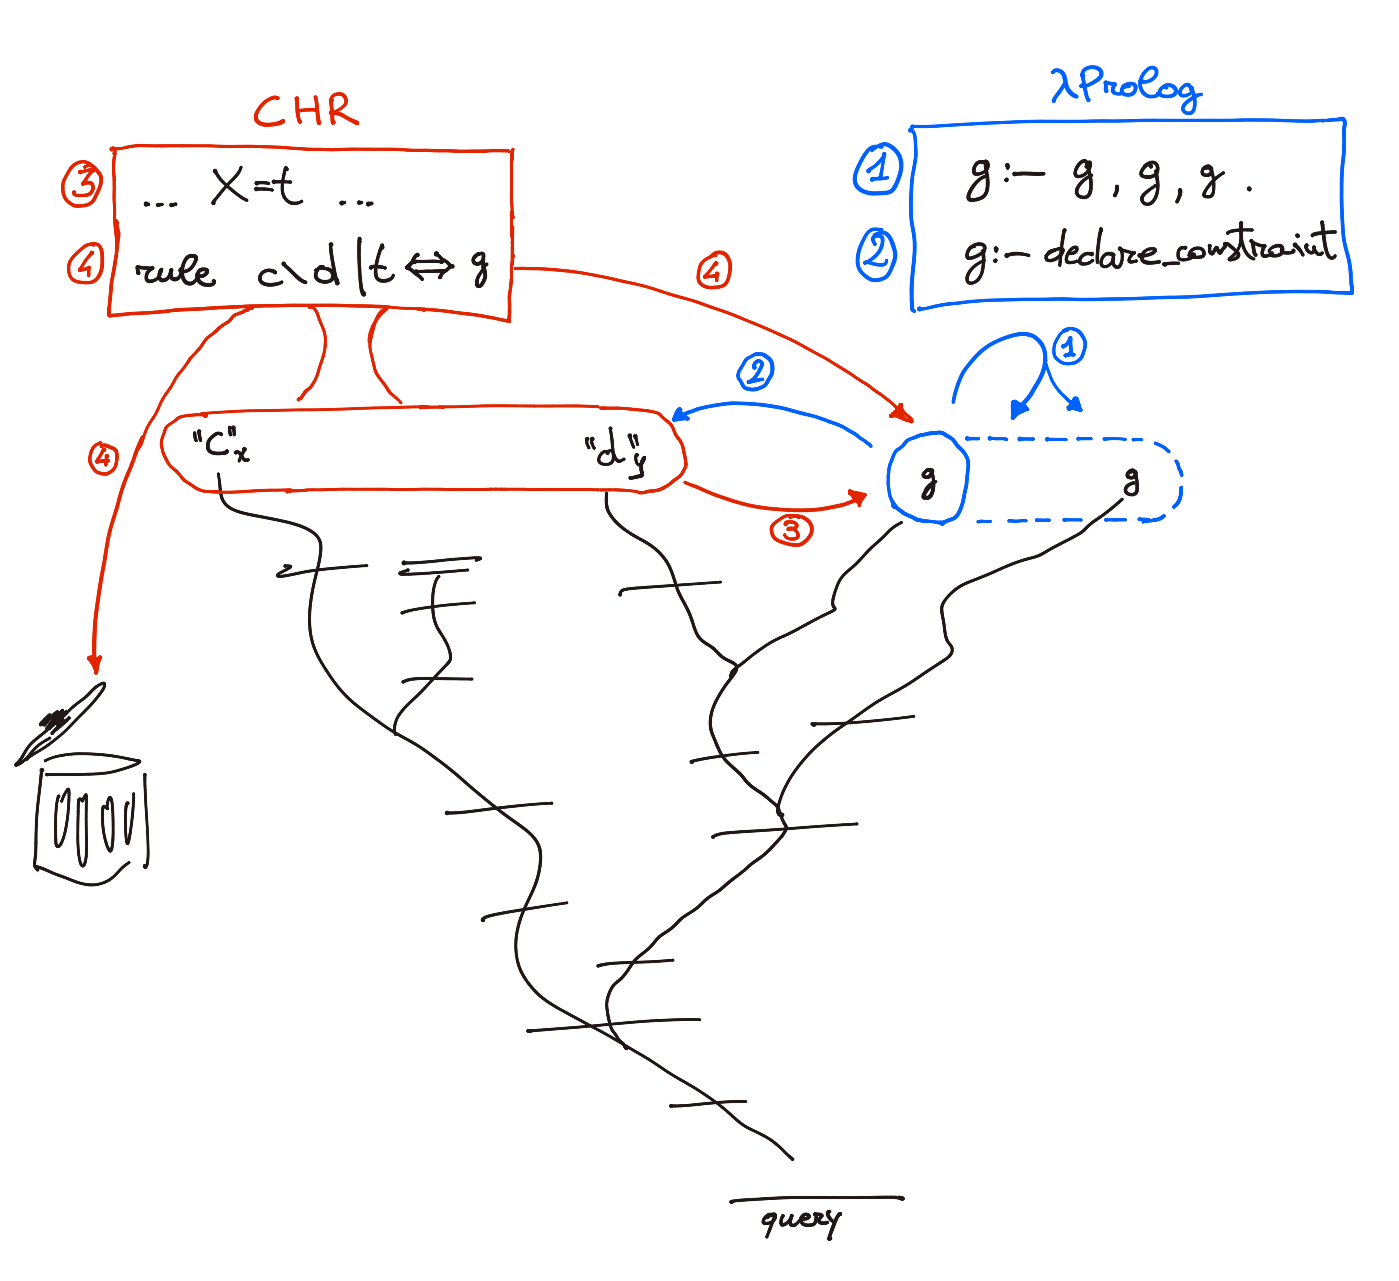
\includegraphics[width=0.8\textwidth]{chr.png}
%  \caption{\label{chr:fig}Elpi runtime (TODO clause/rule)}
%\end{figure}


\subsection{Abstract syntax and operational semantics}\label{sec:sem}

The objective of this section is to act as a reference for
the semantics of Elpi.

\newcommand{\vecL}[1]{\overrightarrow{\vphantom{t}#1}}
\newcommand{\BASE}{\ensuremath{\mathbb{B}}}
\newcommand{\PRED}[1][]{\ensuremath{\mathbb{F}#1}\xspace}
\newcommand{\VAR}[1][]{\ensuremath{\mathbb{V}#1}\xspace}
\newcommand{\APP}[1][]{\ensuremath{\mathbb{Ap}#1}\xspace}
% \def\CALL{\APP}
\newcommand{\X}[1][]{\ensuremath{\mathcal{X}#1}\xspace}
\newcommand{\T}[1][]{\ensuremath{tm#1}\xspace}
\newcommand{\V}[1][]{\ensuremath{\mathcal{V}#1}\xspace}
\newcommand{\CHR}[1][]{\ensuremath{\mathbb{C}#1}\xspace}
\newcommand{\CLAUSE}[1][]{\ensuremath{\mathbb{R}}#1\xspace}
\newcommand{\ATOM}[1][]{\ensuremath{\mathbb{A}#1}\xspace}
\newcommand{\A}[1][]{\ensuremath{\mathbb{A}#1}\xspace}
\newcommand{\Ainst}[1][]{\ensuremath{\alpha#1}\xspace}
\newcommand{\bool}[1][]{b}
\newcommand{\B}[1][]{\ensuremath{\mathrm{B}}\xspace}
\newcommand{\F}[1][]{\ensuremath{\mathbb{D}}\xspace}
\newcommand{\subst}[1][]{\ensuremath{\sigma#1}\xspace}
\newcommand{\alt}[1][]{\ensuremath{\mathcal{A}#1}\xspace}
\newcommand{\alts}[1][]{\ensuremath{a#1}\xspace}
\newcommand{\g}[1][]{\ensuremath{\mathcal{G}#1}\xspace}
\newcommand{\clause}[1][]{\ensuremath{\mathcal{@}#1}\xspace}
\newcommand{\pred}[1][]{\ensuremath{p#1}\xspace}
\newcommand{\expr}[1][]{\texttt{e#1}\xspace}
\newcommand{\vars}{\texttt{vars}}
\newcommand{\run}{\texttt{run}}
\newcommand{\fold}{\ensuremath{\mathbf{fold}}\xspace}
\newcommand{\map}{\ensuremath{\mathbf{map}}\xspace}
% \newcommand{\fail}{\texttt{fail}}
\newcommand{\call}{\texttt{Call}}
\newcommand{\cut}{\texttt{Cut}\xspace}
\newcommand{\cst}{\texttt{Cst}\xspace}
%\newcommand{\goal}{\texttt{Goal}}
\newcommand{\unifiable}{\texttt{unifiable}\xspace}
\newcommand{\matchable}{\texttt{matchable}\xspace}
\newcommand{\nUnify}{\texttt{split}\xspace}
\newcommand{\unify}{\texttt{unify}\xspace}
\newcommand{\match}{\texttt{match}\xspace}
\newcommand{\impl}{\texttt{=>}}
\newcommand{\prog}[1][]{\ensuremath{{\pi}#1}\xspace}
\newcommand{\pin}{\texttt{pi}}
\newcommand{\cdash}{\texttt{:-}} % colon-dash
\newcommand{\Cons}[1]{\ensuremath{#1::}}
\newcommand{\ConsHd}[1]{\ensuremath{(#1::}\xspace}
\newcommand{\ConsTl}[1]{\ensuremath{#1)}\xspace}
\newcommand{\EmptyList}{\ensuremath{\varnothing}}
\newcommand{\ConsHdNP}[1]{\ensuremath{#1::}\xspace}
\newcommand{\ConsTlNP}[1]{\ensuremath{#1}\xspace}

\newcommand{\EmptySubst}{\ensuremath{\varepsilon}}

\newcommand{\PROG}[1][]{\ensuremath{\mathcal{P}#1}\xspace}
\newcommand{\progCut}{\ensuremath{\prog[^!]}\xspace}
\newcommand{\evdash}{\ensuremath{\colondash}\xspace}
\newcommand{\piimpl}{{\ensuremath{\forall\Rightarrow}}\xspace}
\newcommand{\TYPE}[1][]{\ensuremath{\mathbb{T\!y}#1}}
\newcommand{\TERM}[1][]{\ensuremath{\mathbb{T\!m}#1}}
\newcommand{\SIGN}[1][]{\ensuremath{\mathbb{S}#1}}
\newcommand{\func}[1][]{\ensuremath{\mathcal{D}#1}}
\newcommand{\implCmd}[2]{\ensuremath{#1\ \impl\ #2}}
\newcommand{\bchain}{\ensuremath{\mathcal{B}}}
\newcommand{\cselect}{\ensuremath{\mathcal{U}}}
% \newcommand{\bs}{\text{\textbackslash}}
\newcommand{\bs}{\text{.}}
\newcommand{\piCmd}[2]{\ensuremath{\pin\ #1 \bs\ #2}}
% \newcommand{\piImplCmd}[3]{\piCmd{#1}{\implCmd{#2}{#3}}}
\newcommand{\ground}{\texttt{ground}}
\newcommand{\dom}{\texttt{vars}}
\newcommand{\clauseCmd}[3]{\ensuremath{#1\ #2\ \cdash\ #3}}

We assume a set \PRED of functors (term/predicate constructors), and a set \VAR of term variables
($X,Y,\ldots$ for unification variables and $x,y,\ldots$ for bound variables).
% The non-terminal \CALL groups callable symbols ($c,d,\ldots$): either predicate names or variables.

In the syntax of atoms \ATOM we single out \cut and \cst.
The \cut operator corresponds to \elpi{!} in the concrete syntax.
The \cst one corresponds to \elpi{declare_constraint} in the concrete syntax
and it carries the applicative term to suspend and the list of variables triggering
its resumption.

%The non-terminal $\TERM$, for terms, includes predicate calls, functor applications and $\lambda$-abstraction.
% For simplicity we glue together the
% \elpi{pi} and \elpi{=>} in the same grammar production and we
% rule out predicates inside data (like lists of predicates).

%for regular data or \V{} for 
% and polymorphic data.
% We note $\Ainst \in \A$.
% The usual =/2 operator is
% encoded as a regular predicate \texttt{eq} with a single clause
% \elpi{(eq X X :- .)} and signature\todo{dire che poly è solo su exp}
% $\ctx\ \texttt{eq} = \dtype{\detI}{}{\expI\ \expI}$: a deterministic predicate\todo{should add var to static check}
% with two outputs of the same type.
We write \(\vecL{t}\) to denote \(t_1 \ldots t_n\) i.e. a (possibly
empty) list of \(t\)s.
Similarly, we write \(\vecL{tu}\) to denote the
element-wise pairing (zipping) of \(\vecL{t}\) and \(\vecL{u}\) into a list of
pairs. %The zipping process continues up to the length of the shorter list.
% \todo{check for dead cod here if we hide the proofs}

We write
$t[x/y]$ for the usual, capture avoiding, operation of replacing the variable $x$
with $y$ inside $t$.
% We say that $\vars\ t$ is the set
% of free variables occurring in $t$ (the binders are \elpi{pi} and $\lambda$).
% When $\vars\ t = \EmptyList$ we say that
% $t$ is \ground.

% We call \emph{toplevel clauses} the ones that are in the initial program.
% %or equivalently that are asserted by the atoms in the query. 
% We call
% \emph{hypothetical clauses} the ones that are asserted by atoms in the premises
% of a clause.

\begin{figure}
  $$
  \begin{array}{rlr}
    \PRED & ::= p, q, \ldots, f, g, \ldots & \mathrm{functors}\\
    \VAR & ::= \mathrm{X}, \mathrm{Y} \ldots x, y, \ldots & \mathrm{variable}\\
    \APP & ::= \PRED\ \vecL{\TERM} \mid  \VAR\ \vecL{\TERM} & \mathrm{applicative}\\
    \ATOM& ::= \cut \mid \cst\ \APP\ \vecL{\VAR} \mid \APP \mid \piCmd{\VAR}{\ATOM} \mid \implCmd{{\CLAUSE}}{\ATOM} & \mathrm{atom} \\
    \TERM & ::= \APP \mid \lambda \VAR \bs\ \TERM & \mathrm{term}\\
    \CLAUSE & ::= \clauseCmd{\APP}{\!}{\vecL{\ATOM}} & \mathrm{logic\ programming\ rule}\\
    \CHR & ::= \vecL{\APP}\ \backslash\ \vecL{\APP}\ 
               \mathrm{|}\ \APP \Leftrightarrow  \vecL{\APP} & \mathrm{constraint\ rule}
  \end{array}
  $$
  \caption{Abstract syntax}
  \label{fig:syntax}
\end{figure}

\newenvironment{myRule}[1]{%
  \begin{minipage}{.9\textwidth}
    \centering
    \begin{prooftree}%
      } % Here will be put the body
      {
    \end{prooftree}
    \vspace{2pt}
  \end{minipage}
}
\newcommand{\arr}{\ensuremath{\rightsquigarrow}}
\newcommand{\atsign}{\ensuremath{\mbox{\footnotesize\raisebox{-1pt}{\ensuremath{@}}}}}
\makeatletter
\newcommand{\customlabel}[2]{%
  \protected@write \@auxout {}{\string \newlabel {#1}{{\ensuremath{#2}}{\thepage}{#2}{#1}{}} }%
  \hypertarget{#1}{\ensuremath{#2}}
}
\makeatother
\newcommand{\Keyword}[1]{\texttt{{\fontfamily{qcr}\selectfont #1}}}

\newcommand{\kIF}{\Keyword{if}}
\newcommand{\kTHEN}{\Keyword{then}}
\newcommand{\kELSE}{\Keyword{else}}
\newcommand{\kAS}{\Keyword{as}}
\newcommand{\runCmdR}[3]{\ensuremath{\run\ (k,\ #3,\ #1)\ #2 \arr r}}
\newcommand{\runCmdRK}[4]{\ensuremath{\run\ (#4,\ #3,\ #1)\ #2 \arr r}}
\newcommand{\runCmd}[7]{\ensuremath{\run\ (#4,\ #3,\ #1)\ #2 \arr (#7,\ #6,\ #5)}}
%\newcommand{\runCmdQ}[4]{\ensuremath{\run\ #1\ #2 \arr (#3, #4)}}
\newcommand{\runCmdQR}[2]{\ensuremath{\run\ #1\ #2 \arr r}}
\newcommand{\runQuery}[2]{\ensuremath{\run\ (\EmptySubst,\ \EmptySubst,\ #1)\ #2 \arr \_}}
\newcommand{\runCmdF}[3]{\ensuremath{\run\ (k,\ #3,\ #1)\ #2 \arr \bot}}
% \newcommand{\callCmd}[3]{\ensuremath{(\call\ #1\ #2\ #3)}\xspace}
\newcommand{\callCmd}[2]{\ensuremath{(#1\ #2)}\xspace}
\newcommand{\goalCmd}[3]{\ensuremath{(#1,\ #2,\ #3)}\xspace}
\newcommand{\ruleName}[2]{\customlabel{#1}{\ensuremath{\mathrm{run}_{#2}}}}
\newcommand{\RightLabelM}[1]{\RightLabel{\scriptsize #1}}

\newcommand{\ruleFail}{\ruleName{rule:backtrack}{\circlearrowright }}
\newcommand{\ruleAbort}{\ruleName{rule:abort}{\bot}}
\newcommand{\ruleCall}{\ruleName{rule:call}{@}}
\newcommand{\ruleCallF}{\ruleName{rule:callbacktrack}{\circlearrowright}}
\newcommand{\ruleCallFH}{\ruleName{rule:callabort}{\bot}}
% \newcommand{\ruleCallB}{\ruleName{rule:call1}{@'}}
\newcommand{\ruleBeta}{\ruleName{rule:beta}{\sigma}}
\newcommand{\ruleBang}{\ruleName{rule:cut}{!}}
\newcommand{\ruleCst}{\ruleName{rule:delay}{\bigtriangleup}}
\newcommand{\ruleTcs}{\ruleName{rule:resume}{\bigtriangledown}}
% \newcommand{\ruleCHR}{\customlabel{rule:chr}{\ensuremath{\mathrm{run}_*}}}
\newcommand{\ruleStop}{\ruleName{rule:stop}{\top}}
\newcommand{\ruleUnif}{\ruleName{rule:unif}{=}}
\newcommand{\ruleImpl}{\ruleName{rule:impl}{\Rightarrow}}
\newcommand{\rulePi}{\ruleName{rule:pi}{\forall}}
\newcommand{\ruleMatch}{\ruleName{rule:match}{m}}
\newcommand{\rulePiImpl}{\ruleName{rule:piimpl}{{\piimpl}}}

\newcommand{\ruleStopM}[1]{
  \begin{myRule}{#1}
    % STOP
    \AxiomC{\phantom{\ensuremath{\bchain}}}
    \RightLabelM{\ruleStop}
    \UnaryInfC{\runCmd{\EmptyList}{\alts}{\subst}{\kappa}{\alts}{\subst}{\kappa}}
  \end{myRule}
}

% \newcommand{\ruleUnifM}[1]{
%   \begin{myRule}{#1}
%     % UNIF
%     \AxiomC{\unifyCmd{x}{y}{\subst}{\subst[']}}
%     \AxiomC{\runCmdR{\vecL{g}}{\alts}{\subst[']}}
%     \RightLabelM{\ruleUnif}
%     \BinaryInfC{\runCmdR{\ConsHdNP{\goalCmd{\_}{x = y}{\_}}\ConsTlNP{\vecL{g}}}{\alts}{\subst}}
%   \end{myRule}
% }

% \newcommand{\ruleMatchM}[1]{
%   \begin{myRule}{#1}
%     % MATCH
%     \AxiomC{\matchCmd{x}{y}{\subst}{\subst[']}}
%     \AxiomC{\runCmd{\vecL{g}}{\alts}{\subst[']}{\alts[']}{\subst['']}}
%     \RightLabelM{\ruleMatch}
%     \BinaryInfC{\runCmd{\ConsHdNP{\goalCmd{\_}{(x =_m y)}{\_}}\ConsTlNP{\vecL{g}}}{\alts}{\subst}{\alts[']}{\subst['']}}
%   \end{myRule}
% }

\newcommand{\ruleFailM}[1]{
  \begin{myRule}{#1}
    % FAIL
    \AxiomC{\unifyCmd{x}{y}{\subst}{\bot}}
    \AxiomC{\runCmdQR{\alts}{al}}
    \RightLabelM{\ruleFail}
    \BinaryInfC{\runCmdR{\ConsHdNP{\goalCmd{\_}{x = y}{\_}}\ConsTlNP{\_}}{\ConsHd{\alts}\ConsTl{al}}{\subst}}
  \end{myRule}%
}

\newcommand{\ruleAbortM}[1]{
  \begin{myRule}{#1}
    % FAIL
    \AxiomC{\unifyCmd{x}{y}{\subst}{\bot}}
    \RightLabelM{\ruleAbort}
    \UnaryInfC{\runCmdF{\ConsHdNP{\goalCmd{\_}{x = y}{\_}}\ConsTlNP{\_}}{\EmptyList}{\subst}}
  \end{myRule}%
}

\newcommand{\ruleBangM}[1]{
  \begin{myRule}{#1}
    % CUT
    \AxiomC{\runCmdR{\vecL{g}}{\alts}{\subst}}
    \RightLabelM{\ruleBang}
    \UnaryInfC{\runCmdR{\ConsHdNP{\goalCmd{\_}{\cut}{\alts}}\ConsTlNP{\vecL{g}}}{\_}{\subst}}
  \end{myRule}
}
\newcommand{\ruleCstM}[1]{
  \begin{myRule}{#1}
    % suspend
    \AxiomC{\ensuremath{\mathcal{CHR}(k,\ \prog,\ c,\ t,\ \alts[']) = (\vecL{g'}, k')}}
    \AxiomC{\runCmdRK{\vecL{g'} \atsign \vecL{g}}{\alts}{\subst}{k'}}
    \RightLabelM{\ruleCst}
    \BinaryInfC{\runCmdRK{\ConsHdNP{\goalCmd{\prog}{\cst\ c\ t}{\alts[']}}\ConsTlNP{\vecL{g}}}{a}{\subst}{k}}
  \end{myRule}
}
\newcommand{\ruleTcsM}[1]{
  \begin{myRule}{#1}
    % resume
    \AxiomC{
      \ensuremath{
        \begin{array}{c}
      (\prog,\ c,\ t) \in k \quad \exists v \in t, v \in \dom\ \subst\\
      \runCmdRK{\ConsHdNP{(\prog,\ c,\ a)}\vecL{g}}{\alts}{\subst}{k - (\prog,\ c,\ t)}
        \end{array}
      }
    }
    \RightLabelM{\ruleTcs}
    \UnaryInfC{\runCmdRK{\vecL{g}}{a}{\subst}{k}}
  \end{myRule}
}
% \newcommand{\ruleCHRM}[1]{
%   \begin{myRule}{#1}
%     % CHR
%     \AxiomC{\ensuremath{\mathcal{CHR}\ m = (\vecL{g'}, m')}}
%     \AxiomC{\runCmdR{\vecL{g'} \atsign \vecL{g}}{\alts}{(s,m')}}
%     \RightLabelM{\ruleCHR}
%     \BinaryInfC{\runCmdR{\vecL{g}}{\alts}{(s,m)}}
%   \end{myRule}
% }

\newcommand{\ruleCallM}[1]{
  \begin{myRule}{#1}
    % CALL
    \AxiomC{$\bchain(\prog, \pred\ \vecL{t}, \vecL{g}, \subst, al) = \ConsHdNP{\alts[']}\ConsTlNP{al'}$}
    \AxiomC{\runCmdQR{\alts[']}{(al'\ \atsign\ al)}}
    \RightLabelM{\ruleCall}
    \BinaryInfC{\runCmdR{\ConsHdNP{\goalCmd{\prog}{\callCmd{\pred}{\vecL{t}}}{\_}}\ConsTlNP{\vecL{g}}}{al}{\subst}}
  \end{myRule}
}
\newcommand{\ruleCallMF}[1]{
  \begin{myRule}{#1}
    % CALL
    \AxiomC{$\bchain(\prog, \pred\ \vecL{t}, \vecL{g}, \subst, a::al) = \EmptyList$}
    \AxiomC{\runCmdQR{a}{al}}
    \RightLabelM{\ruleCallF}
    \BinaryInfC{\runCmdR{\ConsHdNP{\goalCmd{\prog}{\callCmd{\pred}{\vecL{t}}}{\_}}\ConsTlNP{\vecL{g}}}{(a :: al)}{\subst}}
  \end{myRule}
}
\newcommand{\ruleCallMFH}[1]{
  \begin{myRule}{#1}
    % CALL
    \AxiomC{$\bchain(\prog, \pred\ \vecL{t}, \vecL{g}, \subst, \EmptyList) = \EmptyList$}
    \RightLabelM{\ruleCallFH}
    \UnaryInfC{\runCmdF{\ConsHdNP{\goalCmd{\prog}{\callCmd{\pred}{\vecL{t}}}{\_}}\ConsTlNP{\vecL{g}}}{\EmptyList}{\subst}}
  \end{myRule}
}

\newcommand{\ruleCallBeta}[1]{
  \begin{myRule}{#1}
    \AxiomC{$\subst (X\ \vecL{t}) =_{\beta\eta} \pred\ \vecL{u}$}
    \AxiomC{\runCmdR{\ConsHdNP{\goalCmd{\prog}{\pred\ \vecL{u}}{a}}\ConsTlNP{\vecL{g}}}{\alts[']}{\subst}}
    \RightLabelM{\ruleBeta}
    \BinaryInfC{\runCmdR{\ConsHdNP{\goalCmd{\prog}{(X\ \vecL{t})}{a}}\ConsTlNP{\vecL{g}}}{\alts[']}{\subst}}
  \end{myRule}
}


% \newcommand{\ruleCallBM}[1]{
%   \begin{myRule}{#1}
%     % CALLB
%     \AxiomC{$(\subst h)\ \vecL{t} =_\beta \pred\ \vecL{u}$}
%     \AxiomC{$\bchain(\prog, \pred\ \vecL{u}, \subst, \alts) = \ConsHdNP{g}\ConsTlNP{new\_alt}$}
%     \AxiomC{\runCmdR{(g\ \atsign\ \vecL{g})}{(new\_alt\ \atsign\ \alts)}{\subst}}
%     \RightLabelM{\ruleCallB}
%     \TrinaryInfC{\runCmdR{\ConsHdNP{\goalCmd{\prog}{(h\ \vecL{t})}{\_}}\ConsTlNP{\vecL{g}}}{\alts}{\subst}}
%   \end{myRule}
% }

\newcommand{\env}{\ensuremath{\mathcal{E}}}

\newcommand{\ruleImplM}[1]{
  \begin{myRule}{#1}
    % IMPL
    \AxiomC{\ensuremath{\runCmdR{\ConsHdNP{\goalCmd{(h + \prog)}{g}{\alts}}\ConsTlNP{\vecL{g}}}{\alts[']}{\subst}}}
    \RightLabelM{\ruleImpl}
    \UnaryInfC{\ensuremath{\runCmdR{\ConsHdNP{\goalCmd{\prog}{(\implCmd{h}{g})}{\alts}}\ConsTlNP{\vecL{g}}}{\alts[']}{\subst}}}
  \end{myRule}
}

\newcommand{\rulePiM}[1]{
  \begin{myRule}{#1}
    % PI
    \AxiomC{\ensuremath{y \# \prog \quad \runCmdR{\ConsHdNP{\goalCmd{(y + \prog)}{g[x/y]}{\alts}}\ConsTlNP{\vecL{g}}}{\alts[']}{\subst}}}
    \RightLabelM{\rulePi}
    \UnaryInfC{\ensuremath{\runCmdR{\ConsHdNP{\goalCmd{\prog}{(\piCmd{x}{g})}{\alts}}\ConsTlNP{\vecL{g}}}{\alts[']}{\subst}}}
  \end{myRule}
}

% \newcommand{\rulePiImplM}[1]{
%   \begin{myRule}{#1}
%     % IMPL
%     \AxiomC{$y \# \prog$}
%     \AxiomC{\runCmdR{\ConsHdNP{\goalCmd{(y,h[y/x]) + \prog}{g[y/x]}{\alts}}\ConsTlNP{\vecL{g}}}{\alts[']}{\subst}}
%     \RightLabelM{\rulePiImpl}
%     \BinaryInfC{\runCmdR{\ConsHdNP{\goalCmd{\prog}{(\piCmd{x}{\implCmd{h }{g}})}{\alts}}\ConsTlNP{\vecL{g}}}{\alts[']}{\subst}}
%   \end{myRule}
% }


\newcommand{\unifyCmd}[5][]{\ensuremath{
  \ifstrequal{#1}{1}
    {\vecL{\unify\ #2\ #3}}
    {\unify\ #2\ #3}\ #4 = #5}}
\newcommand{\matchCmd}[5][]{\ensuremath{
  \ifstrequal{#1}{1}
  {\vecL{\match\ #2\ #3}}
  {\match\ #2\ #3}\ #4 = #5}}

We use $\EmptyList$ for the empty list and $x :: xs$ for prepending an element $x$
to a list $xs$; $\atsign$ for list concatenation;
$[e\ \kIF\ p\ |\ x \in \vec{x}]$ for list comprehension (we omit the filter when $p$ is true).

\noindent

We denote with $\_\times\_$, $\_+\_$, $\vecL{\phantom{i}\_~}$ and $\_\to\_$ the product, disjoint union, list and
function space of types, respectively, and with $\B = \{ \top, \bot\}$ the booleans.
% We omit the conversion between the (isomorphic) types $A \times B \to C$
% and $A \to B \to C$, e.g. we may write $\map\ f\ \vecL{tu}$ instead of $\map\ (\lambda x.f\ (\text{fst}\ x)\ (\text{snd}\ x))\ \vecL{tu}$.

A substitution $\subst$ of type $\Sigma$
%is a pair $(s,m)$ where $s$ 
is a mapping from unification variables
\VAR to terms \TERM{}. % and $m$ is a constraint store.
We write
% $s\ t$ the application of the substitution $s$ to a term $t$, and 
$\subst\ t$ the  application of the substitution to $t$.
%the first component of \subst to $t$.
% ,
% and we remark that $t$ is \ground{} iff $\forall \subst, \subst t = t$.
We write $\dom\ \subst$ for the set of variables occurring
in the domain %or in the codomain 
of \subst, i.e.
$\dom\ \subst = \{ X\ |\ \subst X \mathrm{\ is\ defined\ }\}$. % \lor X \in \vars\ (\subst Y) \mathrm{\ for\ some\ Y} \}$.
The empty substitution is written $\EmptySubst$. % is so that $\dom\ \EmptySubst = \EmptyList$.

We assume a function $\unify$ of type $\TERM \times \TERM \times \Sigma \to \Sigma + \bot$
such that if $\unifyCmd{t_1}{t_2}{\subst}{\subst[']} \not= \bot$ 
then \subst['] is the most general extension of \subst 
such that $\subst['] t_1 = \subst['] t_2$.
We assume a function $\match$ of type $\TERM \times \TERM \times \Sigma \to \Sigma + \bot$
such that if $\matchCmd{t}{p}{\subst}{\subst[']} \not= \bot$
then \subst[']  is the most general extension of  $\subst$
such that $\subst t = \subst['] p$ and $\subst[']t = \subst t$,
i.e. \match{} does not assign variables in $t$ but only in $p$ that acts as the pattern.

A program $\prog$ of type $\PROG$ is a pair $(\mathbb{N}, \mathcal{I})$
where $\mathbb{N}$ is a set of names and $\mathcal{I}$ an index
mapping predicate names to an \emph{ordered list} of rules.
We write $x \# \prog$ to find a name fresh in $\mathbb{N}$.
We write $\prog~\pred$ for the clauses of predicate \pred in $\mathcal{I}$
and we write $x + \prog$ to add the name $x$ to $\mathbb{N}$
and we write $h + \prog$ to prepend the extra clause $h$  to $\mathcal{I}$
(hence $h$ has the highest priority in the new program).

A constraint store $\kappa$ of type $K = \vecL{\PROG \times \APP \times \vecL{\VAR}}$
is a multiset of triples $(\prog,c,t)$
where $\prog$ is a program, where $c$ stands for a constraint (an applicative term in $\APP$) and $t$
of type $\vecL{\VAR}$ is the trigger. The empty store is written $\EmptySubst$;
we use $k - (\prog,c,t)$ to remove a constraint from the store.

A goal $g$ of type $\g = \PROG \times \ATOM \times \vecL{\alt}$
is a triple made of a program, an atom and a list of
so called \emph{cut-to} alternatives.
An alternative $a$ of type $\alt$ is a triple of type $K \times \Sigma \times \vecL{\g}$
made of a constraint store, a substitution and a list of goals.

\begin{figure}[!]
    \centering

  % \ruleCHRM{.4}
  \ruleCstM{.4}
  \ruleTcsM{.4}
  \caption{Semantics: constraints}
    \label{fig:basic-interp-c}
\end{figure}

  \begin{figure}[!]
  \centering
  \ruleStopM{.37}
  \ruleCallMFH{0.44}
  \ruleCallMF{0.58}
  % \vspace{0.3em}%
  \ruleBangM{.4}
  \ruleCallM{1}
%


  \rulePiM{1}
  \ruleImplM{1}
  \ruleCallBeta{1}
  
  \caption{Semantics: logic programming}
    \label{fig:basic-interp-l}
\end{figure}


The operational, big step, semantics of Elpi is given by the function
$$
\run{} : \alt \times \vecL{\alt} \to (K  \times \Sigma \times \vecL{\alt}) + \bot
$$
in Figures~\ref{fig:basic-interp-c} and~\ref{fig:basic-interp-l}.
We write \runCmd{\vecL{g}}{a}{\subst}{\kappa}{a'}{\subst'}{\kappa'}
when a goal list $\vecL{g}$ in a constraint store $\kappa$ and under a substitution \subst and alternatives $a$
terminates with an updated constraint store $\kappa'$, a substitution $\subst'$ and a remaining list of
(still unexplored) alternatives $a'$. We write  \runCmdF{\vecL{g}}{a}{\subst}
when the execution halts: fails to solve one of the given goals and runs out of
alternatives. 
%An initial query looks like \runQuery{[\goalCmd{\prog}{\pred\ \vecL{t}}{\EmptyList}]}{\EmptyList}

Rules in Figures~\ref{fig:basic-interp-c} and~\ref{fig:basic-interp-l}
are applied in the given order. Rules~\ref{rule:suspend} and~\ref{rule:resume}
cover the constraint part of the language: the former updates the constraint
store when a new constraint is declared, while the latter resume a constraint
as soon as the substituion \subst acts on its trigger.

Rule~\ref{rule:stop} applies when all goals are solved and returns
the substitution along with the still unexplored alternatives.
Rule~\ref{rule:callabort} applies when no rule applies to the
current goal and not alternative is avilable.
Rule~\ref{rule:callbacktrack} implements (chronological) backtracking by simply
popping the last alternative (going back to the most recent choice point).
Rule~\ref{rule:cut} implements a hard cut by restoring the cut-to alternatives
saved by $\bchain$ (see its description below).
Rule~\ref{rule:call} backchains all applicable rules generating new
alternatives, the first one of which becomes the new goal.
Rule~\ref{rule:beta} takes into account the higher order programming part
of $\lambda$Prolog: unification variables can be used to pass
predicates around.
Rule~\ref{rule:pi} introduces a fresh name into the program
while rule~\ref{rule:impl} introduces a new rule into the program.

\paragraph{Definition of $\bchain$ (backchain)}

The role of $\bchain$ of type $K \times \APP \times \vecL{\g} \times \Sigma \times \vecL{\alt} \to \vecL{\alt}$ is to generate
an alternative for each rules that applies to the given goal.

  $$
  \begin{array}{l}
  \bchain(\prog,\ \pred\, \vecL{t},\ \vecL{g},\ \subst,\ a) =\\
  \qquad
  \bigg[
    %\bigg(
    \subst['],
    %\Big(
    %\underbrace{
      \big(\big[(\prog, g, a) \mid g \in\! \vecL{b}\big] \atsign\ \vecL{g}\big)
    %}_{\mathrm{premises}} \atsign ~ \vecL{g}
    \ \kIF\ \cselect(\vecL{tu}, \subst) = \subst['] \not= \bot
    %\Big)
    %\bigg)
    ~\bigg|~
    (\clauseCmd{\pred}{\vecL{u}}{\vecL{b}}) \in \prog\ \pred
    \bigg]\vspace{1em}
  \end{array}
  $$

It is worth pointing out that each new goal (in each alternative)
carries the same cut-to alternative and that the value passed to
$\bchain$ by rule \ref{rule:call} is the list of alternatives
before the backchaining happened, i.e. it does not contain any
alternative being created nor any alternative created in the future
by exploring the new alternatives.

\paragraph{Definition of $\cselect$ (select)}

Function $\cselect$ is used to filter rules, keeping only the ones the
apply. Unlike standard Prolog, arguments flagged by the user
as input (written $\vecL{tu_i}$) are matched, while
the ones flagges as output (written $\vecL{tu_o}$) are unified.

  $$
  \begin{array}{l}
  \cselect(\vecL{tu}, \subst) = \fold\ \unify\ \vecL{tu_o}\ (\fold\ \match\ \vecL{tu_i}\ \subst)
  \end{array}
  $$
  
The list processing combinator \fold %and \map 
is defined by the following equations:
$$
\begin{array}{lll}
\fold\ \_\ \_\ \bot = \bot & \fold\ f\ (x :: xs)\ a = \fold\ f\ xs\ (f\ x\ a) & \fold\ \_\ \EmptyList\ a = a %\\
% \map\ \_\ \EmptyList = \EmptyList & \map\ f\ (x :: xs) = f\ x :: \map\ f\ xs
\end{array}
$$

\paragraph{Definition of $\mathcal{CHR}$ (simpagation)}
 
Constraint rule application follows the refined operational
semantics~\cite{10.1007/978-3-540-27775-0_7} that amounts to a precise nesting of iterations.

The starting point is the so called ``active constraint'' that, in the context of Elpi, is
the constraint just declared as $\cst\ c\ t$ by the rule~\ref{rule:delay}.

$$
\mathcal{CHR}(k,\ \prog,\ c,\ t,\ \alts) = (\vecL{g}, k')\ \mathrm{where}
$$
\begin{enumerate}
\item add the active constraint $(\prog,\ c,\ t)$ to $k$ to obtain $k'$
\item for each rule $P_1 \ldots P_x\ \backslash\ P_{x+1} \ldots P_n\ |\ Q \Leftrightarrow g$
\item for each position $0 < j \leq n$
\item for each permutation of $C_1 \ldots C_n$ constraints in $k'$ having $C_j = (\prog,\ c,\ t)$
\item match all $C_i$ with $P_i$ and run $Q$. If it succeeds:
  \begin{itemize}
    \item remove $C_{x+1} \ldots C_n$ from $k'$
    \item remove all permutations involving $C_{x+1} \ldots C_n$
    \item add $g$ to $\vecL{g}$
  \end{itemize}
\item move to the next rule
\end{enumerate}

This description how CHR rules update the constraint store is
essentially the standard operational semantics~\cite{10.1007/978-3-540-27775-0_7}
adapted to constraints that are composed of a program $\prog$ and
an applicative term $c$. As anticipated in~\ref{sec:modes} adapting CHR to Elpi, or
better its $\lambda$Prolog part, requires some extra care. In particular
a constraint $((\mathbb{N},\mathcal{I}),\ c,\ t)$ represents a $\lambda$Prolog goal:
$$
\mathbb{N} \triangleright  \mathcal{I} \vdash c
$$
\noindent
where $\mathbb{N}$ is the set of nominal constants introduced by \elpi{pi}
and $\mathcal{I}$ is the set of rules available to solve $c$.
Pragmatically, only hypothetical rules are stored in the constraint since all
static rules are common to all constraints. In addition to that the
user can specify a filer to discard rules for predicates of no interest for
the constraint (typically rules for predicates unrelated to $c$).
Moreover, for simplicity, $\mathcal{I}$ is presented as a list: if the
user wants to compare these ``contexts'' as sets he has to implement the
quotienting in the rule's guard $Q$. Once more pragmatically, unless
the user explicitly opts out, step 4 only considers the permutations of
constaints with a trigger that overlaps with the trigger $t$ of the active
constraint: according to our experience this is more often than not what
the user needs and drastically cuts down the number of permutations to consider.
Finally the system enfoces the disjointness of names used in each constraint, that
is step 1 really adds $((\mathbb{N'},\mathcal{I'}),\ c',\ t)$ to $k$
where each name in $\mathbb{N'}$ is fresh in $k$, and where
$\mathcal{I'}$ and $c'$ are obtained by subtituting each name in
$\mathbb{N}$ with the corresponding one in $\mathbb{N}'$.
We point the interested
reader to~\cite{TASSI_2019} for a more formal description of the
operational semantics of the $\mathcal{CHR}$ procedure.

\section{Syntactic sugar}

Elpi features some simple syntactic sugar that is elimated by
the ``compiler'' before running programs.

\subsection{Namespaces}

Elpi code is obtained by accumulating together files, that is
``concatenating'' lists of rules, possibly written by different
authors. It is not impossible that
two files, file1 and file2, contain declarations for a predicate with same name p.

When the types for p do not match, Elpi fails immediately
and the programmer is warned. But when the types match, it may
happen that the predicate changes meaning or complexity,
especially in case of failure.

A simple man solution could be to simply put the file name
as part of predicate names, eg file1.p and file2.p.

To paliate the syntactic overhead Elpi provides two syntactic
facilities: namespace and shorten. The former prefixes all
names of the predicates contained in a block, the latter makes
predicates accessible via a short name inside a file or a block

In the following snippet the predicate \elpi{p} lives in the namespace
\elpi{n} and is hence accessible via the long name \elpi{n.p} (outside of
the name space).

\begin{elpicode}
namespace n {
  pred p.
  p :- ... p ...
}
q :- n.p
\end{elpicode}

Long names can be shortened via the \elpi{shorten} directive.

\begin{elpicode}
shorten n.{ p }. % shortens n.p naming n. implicit
q :- p.
% desugars to: q :- n.p.
\end{elpicode}

\subsection{Spilling}\label{sec:spilling}

We argue that the names we give to the objects we manipulate
are the most important form of documentation and badly chosen
name are the primary cause of unreadable code.

The time a sloppy programmer saves by using \elpi{TMP}, \elpi{AUX}
or \elpi{X'} instead of thinking at an appropriate name is
demanded, with interests, to any reader of code, including himself.

Logic programming, even in its Higher Order flavor, distinguishes
commands from expressions (predicates from data). This characteristic
is the primary contributor to the proliferation of temporary
variables, a phenomenon that functional programming languages
reduce by putting in the same syntactic category function calls an
data. 

For example the OCaml code \texttt{List.rev (List.append l1 l2)}
or its equivalent \texttt{List.append l1 l2 |> List.rev} enables
to programmer to avoid naming the result of append, while in logic
programming one often reads

\begin{elpicode}
code L1 L2 Result :- append L1 L2 TMP, rev TMP Result.
\end{elpicode}

Elpi provides a syntatic facility to let one use
``partially applied'' predicates as ``function calls''.
By partially applied we mean ``applied to all the arguments flagged as input''.
For example the code above can be written as follows

\begin{elpicode}
code L1 L2 Result :- rev {append L1 L2} Result.
\end{elpicode}

The curly braces identify a term to be \emph{spilled} to the closest
\emph{execution point}, identified by walking the terms outside in and
identifying the first expression of type \elpi{prop}.

Spilling can be nested. Its elaboration is akin to the generation
of the administrative normal form that is commonly used in functional
programming languages.

\subsubsection{Spilling under a binder}

When the spilled expression needs to cross a binder in order to
reach the execution point, the elaboration is more sophisticated.
For example: 

\begin{elpicode}
code Result :- Result = (lam x\ {mk-app f [x]}).
code Result :- (pi y\ mk-app f [y] (TMP y)), Result = (lam x\ TMP x).
\end{elpicode}
  

In order to run the spilled code in a context with the bound variable
\elpi{x}, the expression must be put under a \elpi{pi y}. Similarly
the temporary variable needs to be abstracted over the variable, so
that we can identify the original one \elpi{x} with the one abstracted by
\elpi{pi y}.

Note that spilling does not need to cross a \elpi{pi}, but
needs to make the quantified variable visible to the result of
the spilled computation, for example explicilty quantifying it
with a sigma. For example:

\begin{elpicode}
  code L1 L2 Result :- pi x\ rev {append [x|L1] L2} (Result x).
  code L1 L2 Result :- pi x\ sigma TMP\ append [x|L1] L2 TMP, rev TMP (Result x).
\end{elpicode}

\subsubsection{Spilling and impliction}

When the object language features a sophisticated HOAS for the context
(as in \ref{GALLINA}) it may be necessary to augment the context with
the implication operator. For example imagine the \elpi{lam}
term constructor carries the type of the bound variable

\begin{elpicode}
  code Ty Result :- Result = (lam Ty x\ lam {of x Ty => of (app g x)} y\ ...)
  code Ty Result :-
    (pi x\ of x Ty => of (app g x) (TMP x))
    Result = (lam Ty x\ lam (TMP x) y\ ...)
\end{elpicode}

This is frequent when spilling combined with quotations, for example

\begin{elpicode}
  T = {{ λx : nat => lp:{{ app f {api x}  }}  }}
\end{elpicode}

where the api needs the context of the object language, see \ref{FFI}

\paragraph{Spilling ambiguities}

Not all that glitter is gold. Sometimes the closest execution
point may not be what the programmer wants.

\begin{elpicode}
  code D TodoForLater  :-
    TodoForLater [ this, that {rev D} ].
\end{elpicode}

If this and that are predicated, the latter becomes
\elpi{(rev D TMP, that TMP)} meaning that
\elpi{D} is reversed when \elpi{TodoForLater} will be executed, and
not when the todo list is generated, as one may have wanted.

According to our experience the closes execution point
is more often than not what the programmer expects.

\section{A complete example: Hindley Milner type inference}\label{sec:milner}

The most significant type inference algorith is the one crafted by
Milner the ML language~\cite{MILNER1978348}. The flavor we 
study here covers equality type variables, the \texttt{''a} abstraction
(in standard ML syntax) for decidable types, i.e. types that can be
effectively compared unlike the function space.

It makes a good use case for Elpi because:
\begin{itemize}
  \item it manipulates syntax trees with binders, namely lambda abstraction
    and let binding
  \item it manipulates types containing unification variables (i.e. holes).
    The key step in the algorithm is to turn (existentially quantified)
    unification variables into universally quantifies type variables to
    form a skema
  \item unification variables have an attribute, a flag (denoted with
    an over bar) that is set if the equality test is used on values
    of their type.
\end{itemize}

The syntax of terms is very similar to the simply typed $\lambda$-calculus
one, with the addition of \texttt{let} and the equality test. We omit
conditional, loops or recursion since it does not play an important role.

\begin{center}
\begin{minipage}{0.35\textwidth}
$$
\begin{array}{lrl}
  e & =     & x                                 \\
  & \vert & e_1\ e_2                            \\
  & \vert & \lambda\ x\ .\ e                    \\
  & \vert & \mathtt{let}\ x = e_1\ \mathtt{in}\ e_2 \\
  & \vert & e_1 = e_2 \\
\end{array}
$$
\end{minipage}
\begin{minipage}{0.60\textwidth}
\vspace{0.5em}
%elpi:hm.elpi
\begin{elpicodelj}
kind term   type.
type global string -> term.
type app    term -> term -> term.
type lam    (term -> term) -> term.
type let    term -> (term -> term) -> term.
type eq     term -> term -> term.
\end{elpicodelj}
\end{minipage}
\end{center}
~\\  
~\\  
As in section~\ref{sec:hello} we use an HOAS encoding of terms.
Still we add a \elpi{global} term constructor to
be able to set up a minimal environment for our examples.

Monomorphic type expressions $\tau$ and type skemas $\sigma$
are depicted below. As in the original paper we fix a few builtin type contructors
instead of supporting a generic n-ary type former, but unlike
the ML tradition we put type constractors to the left of an application.
We use the infix symbol \elpi{-->} for the function space of ML.

\begin{center}
\begin{minipage}{0.4\textwidth}
$$
\begin{array}{lrl}
  \\
    \tau   &=     & \alpha                    \\
                              &\vert &  \tau \to \tau         \\
                              &\vert &  \mathtt{int}         \\
                              &\vert &  \mathtt{bool}         \\
                              &\vert &  \mathtt{list}\ \tau         \\
                              &\vert &  \mathtt{pair}\ \tau\ \tau         \\
  
     \sigma &=    & \tau                                           \\
                             &\vert& \forall\ \alpha\ .\ \sigma \\
                            &\vert& \forall\ \bar\alpha\ .\ \sigma \\
  \\
\end{array}
$$
\end{minipage}
\begin{minipage}{0.5\textwidth}
%elpi:hm.elpi
\begin{elpicodelj}
kind tye   type.
type (-->) tye -> tye -> tye.  
type int   tye.
type bool  tye.
type list  tye -> tye.
type pair  tye -> tye -> tye.

kind ty     type.
type all    bool -> (tye -> ty) -> ty.
type mono   tye -> ty.
\end{elpicodelj}
\end{minipage}
\end{center}


The typing routing works with a context and, as we did for the
simply typed lambda calculus, we delegate its management to the
programming language.

$$
\begin{array}{llrl}
  \\
    \text{Context}     & \Gamma & = & \epsilon\ \mathtt{(empty)}\\
                       &        & \vert& \Gamma,\ x : \sigma\\
    \text{Typing}      &        & = & \Gamma \vdash e : \sigma\\
  \\
  \end{array}
$$


We give below a fre example of type assignement to global
constants. It is worth highlighting the fact that the
type skema for \elpi{"undup"}


%elpi:hm.elpi
\begin{elpicode}
pred of i:term, o:ty.
of (global "1")      (mono int).
of (global "plus")   (mono (int --> int --> int)).
of (global "nil")    (all ff x\ mono (list x)).
of (global "cons")   (all ff x\ mono (x --> list x --> list x)).
of (global "pr")     (all ff x\ all ff y\ mono (x --> y --> (pair x y))).
of (global "fst")    (all ff x\ all ff y\ mono (pair x y --> x)).
of (global "size")   (all ff x\ mono (list x --> int)).
of (global "undup")  (all tt x\ mono (list x --> list x)).
\end{elpicode}
  

The specialization of type skema allows one to plug type expressions in place
of quantified variables. When the substituted variables stands for an
equality type, one has to check that the type expression has an equality test.

$$
\displaystyle\frac{\tau' = \left\{\alpha_i \mapsto \tau_i\right\} \tau \quad \beta_i \not\in \textrm{free}(\forall \alpha_1...\forall\alpha_n . \tau)}{\forall \alpha_1...\forall\alpha_n . \tau \sqsubseteq \forall \beta_1...\forall\beta_m . \tau'}
$$
$$
\displaystyle\frac{\tau' = \left\{\bar\alpha_i \mapsto \tau_i\right\} \tau \quad \beta_i \not\in \textrm{free}(\forall \alpha_1...\forall\alpha_n . \tau) \quad \overline{eq}(\tau_i)}{\forall \alpha_1...\forall\alpha_n . \tau \sqsubseteq \forall \beta_1...\forall\beta_m . \tau'}
$$
$$
\begin{array}{ll}
  \overline{eq}(\mbox{bool}) & \\
  \overline{eq}(\mbox{int}) & \\
  \overline{eq}(\mbox{list}~\tau) & ~\mbox{if}~ \overline{eq}(\tau) \\
  \overline{eq}(\mbox{pair}~\tau_1~\tau_2) & ~\mbox{if}~ \overline{eq}(\tau_1) ~\mbox{and}~ \overline{eq}(\tau_2)\\
  \overline{eq}(\bar\alpha) & \\
\end{array}
$$

The Elpi code departs from the pen and paper presentation by instantiating, at once,
all skema variables by fresh unification variables, possibly constraining them
to be an eq type

%elpi:hm.elpi
\begin{elpicode}
pred specialize i:ty, o:tye.
specialize (mono T) T.
specialize (all ff F) T :- specialize (F Fresh_) T.
specialize (all tt F) T :- specialize (F Fresh) T, eqbar Fresh.
\end{elpicode}

The \elpi{eqbar} predicate traevrses concrete type expressions and
suspend when variables are found.

%elpi:hm.elpi
\begin{elpicode}
pred eqbar i:tye.
eqbar bool.
eqbar int.
eqbar (list A) :- eqbar A.
eqbar (pair A B) :- eqbar A, eqbar B.
eqbar (uvar as A) :- declare_constraint (eqbar A) [A,_].

constraint of ?- gammabar eqbar theta rm-eqbar {
  rule (eqbar V) \ (theta L) | (not(mem L V)) <=> (theta [V | L]).
}

pred theta i:list tye.
theta L :- declare_constraint (theta L) [_].
\end{elpicode}

The auxiliary constraint \elpi{theta} is used to gather the
(duplicate free) list of unification variables constrained to be equality types.

The use of constraints here is handy but not essential. One could thread a state,
the list of all type variables used so far paired with their equality type status.
The constraint store offers a global state carried on the side of the goals
and constraint handling rules offer the possibility to organize the state, like grouping
all entries into a list.

The declarative code for the type inference algorithm is given below.
The rules for lambda abstraction and application are the same
for simply typed lambda calculus~\ref{inf:stlc}.
The rule for variables finds in $\Gamma$ a skema and assigns to the variable
any valid instance. The rule for let pushes into the context a type
$\overline{\Gamma}(\tau)$ for a let-bound expression of type $\tau$ in $\Gamma$.
Finally the rule for equality tests if the type of the expressions admits
an equality test.

\begin{center}
\begin{minipage}{0.45\textwidth}
$$
\begin{array}{cl}
  \displaystyle\frac{\Gamma \vdash e_0:\tau \rightarrow \tau' \quad\quad \Gamma \vdash e_1 : \tau }{\Gamma \vdash e_0\ e_1 : \tau'}\\ \\
  \displaystyle\frac{\Gamma,\;x:\tau\vdash e:\tau'}{\Gamma \vdash \lambda x.e : \tau \rightarrow \tau'}
\end{array}
  $$
\end{minipage}
\begin{minipage}{0.45\textwidth}
$$
\begin{array}{cl}
  \displaystyle\frac{x:\sigma \in \Gamma \quad \sigma \sqsubseteq \tau}{\Gamma \vdash x:\tau}\\ \\
  \displaystyle\frac{\Gamma \vdash e_0:\tau \quad\quad \Gamma,\,x:\bar{\Gamma}(\tau) \vdash e_1:\tau'}{\Gamma \vdash \mathtt{let}\ x = e_0\ \mathtt{in}\ e_1 :  \tau'}
  \end{array}
$$
\end{minipage}
$$ 
\displaystyle\frac{\Gamma \vdash e_1 : \tau \quad \Gamma \vdash e_2 : \tau \quad \overline{eq}(\tau)}{\Gamma \vdash e_1 = e_2: \mathtt{bool}}
$$
\end{center}

Elpi rules are very close to pen and paper ones. The only difference is that
the rule for variable is extended, on purpose, to any term so that it
can apply to global constants as well.

%elpi:hm.elpi
\begin{elpicode}
of (app H A) (mono T) :-
  of H (mono (S --> T)),
  of A (mono S).

of (lam F) (mono (S --> T)) :-
  pi x\ of x (mono S) => of (F x) (mono T).

of (let E B) (mono TB) :-
  of E (mono T),
  gammabar (mono T) PT,
  pi x\ of x PT => of (B x) (mono TB).

of (eq LHS RHS) (mono bool) :-
  of LHS (mono T),
  of RHS (mono T),
  eqbar T.

of X (mono T) :- of X (all E Poly), specialize (all E Poly) T.
\end{elpicode}

We have already described how \elpi{specialize} relates to $\sqsubseteq$.
What is left to describe is the $\overline{\Gamma}$ operation.
  
$$
\overline{\Gamma}(\tau) = \forall\ \hat{\alpha}\ .\ \tau \quad\quad \hat{\alpha} = \textrm{free}(\tau) - \textrm{free}(\Gamma)
$$

Intuitively one has to compute the free type variables in $\Gamma$ and $\tau$
and only abstract the ones as not free in $\Gamma$, i.e. that are only used
locally to the expressions being bound by the let.

This operation escapes the capabilities of $\lambda$Prolog alone, even with
the mode extensions we discuss in~\ref{sec:modes}, since $\Gamma$ is not
first class or in other words it is automatically managed by the runtime.
This is where the ``meta'' status of constraint handling rules comes in
handy: suspended goals are sequents made of a formula and its context.

%elpi:hm.elpi
\begin{elpicode}
pred gammabar i:ty, o:ty.
gammabar (mono T) TS :- declare_constraint (gammabar (mono T) TS) [_].

constraint of ?- gammabar eqbar theta rm-eqbar {
  rule  \ (theta L)
          (G ?- gammabar T TS)              % matched and removed
        | (generalize L G T POLYT ToRemove) % guard + syntesis
      <=> (TS = POLYT, rm-eqbars ToRemove, theta []). % new goal
  rule \ (eqbar X) (rm-eqbar X).
}

pred rm-eqbars i:list tye.
rm-eqbars [].
rm-eqbars [X|XS] :- rm-eqbar X, rm-eqbars XS.

pred rm-eqbar i:tye.
rm-eqbar X :- declare_constraint (rm-eqbar X) [X, _].

pred generalize i:list tye, i:list prop, i:ty, o:ty, o:list tye.
generalize Theta Gamma (mono T) PolyT ToQuantify :-
  free-ty (mono T) [] VT,
  free-gamma Gamma [] VGamma,
  filter VT (x\ not(mem VGamma x)) ToQuantify,
  bind ToQuantify Theta T PolyT.
\end{elpicode}

\noindent
The code to implement $\overline{\Gamma}(\tau)$ performs thwo tasks:

\begin{itemize}
  \item It abstracts \elpi{T} into a skema \elpi{POLYT} and
    returns is by assigning \elpi{TS}
  \item It cleans up the store of constraints removing the \elpi{eqbar}
    constraints on variables that are now bound in the skema, and updates
    \elpi{theta} by recomputing it
\end{itemize}

The first task is necessary while the second one is mainly to explain an motivate
the scheduling choices described in~\ref{sec:elpiLP+CHR}. In particular it is crucial
that all unneeded \elpi{eqbar} constraints are removed before
\elpi{theta} is recomputed by combining the new constraint with all
\elpi{eqbar} constraints still in the store. It is also worth notion how
the (declarative) semantics of CHR grants that the new \elpi{theta}
constraints is combined with all \elpi{eqbar} ones, no matter in
which order they are added to the store: up to now \elpi{theta} was
there and was updated at every \elpi{eqbar} addition; now all
\elpi{eqbar} are there, and \elpi{theta} gets added and combined
with the all.

The definition of free type variables, Figure~\ref{img:free}, is not
surprising but it is worth to point out two details of the corresponding Elpi code.

\begin{figure}
$$
\begin{array}{ll}
  \text{free}(\ \mathtt{int}\ ) &=\ \emptyset\\
  \text{free}(\ \mathtt{bool}\ ) &=\ \emptyset\\
  \text{free}(\ \mathtt{pair}\ \tau_1\ \tau_2\ ) &=\ \text{free}(\ \tau_1\ )\cup \text{free}(\ \tau_2\ ) \\
  \text{free}(\ \mathtt{list}\ \tau\ ) &=\ \text{free}(\ \tau ) \\
  \text{free}(\ \tau_1 \to \tau_2\ ) &=\ \text{free}(\ \tau_1\ )\cup \text{free}(\ \tau_2\ ) \\
  \text{free}(\ \alpha\ ) &=\ \left\{\alpha\right\}\\
  \text{free}(\ \forall\ \alpha\ .\ \sigma\ ) &=\ \text{free}(\ \sigma\ )\  -\  \left\{\alpha\right\}\\
  \text{free}(\ \Gamma\ ) &=\ \bigcup\limits_{x:\sigma \in \Gamma}\text{free}(\ \sigma\ )\\
\end{array}
$$
\caption{Free type variable\label{img:free}}
\end{figure}

The former is that the context is a list of propositions. The \elpi{prop}
type gather all predicates, not just \elpi{of}. We don't need to add
a rule skip any unrelated predicate the program may have loaded with implication
because the \elpi{constraint of ?- gammabar eqbar theta rm-eqbar} directive
tells Elpi to filter the context of suspended goals (constraint) and keep only
entries for the \elpi{of} predicate.

The second is that, at the meta level of constraint handling rules, the
\elpi{uvar} keyword becomes a regular syntax tree node and that is
has two arguments. The first one is the unique identifier of the unification
variable. The second one is its scope represented as a list of names.
  

%elpi:hm.elpi
\begin{elpicode}
pred free-ty i:ty, i:list tye, o:list tye.
free-ty (mono X) L L1 :- free X L L1.
free-ty (all _ F) L L1 :- pi x\ free-ty (F x) L L1.

pred free-gamma i:list prop, i:list tye, o:list tye.
free-gamma [] L L.
free-gamma [of _ T|X] L L2 :- free-ty T L L1, free-gamma X L1 L2.

pred free i:tye, i:list tye, o:list tye.
free int L L.
free bool L L.
free (list A) L L1 :- free A L L1.
free (pair A B) L L1 :- free B {free A L} L1.
free (A --> B) L L1 :- free B {free A L} L1.
free (uvar _ _ as X) L L1 :- if (mem L X) (L1 = L) (L1 = [X|L]).
\end{elpicode}

The last bit of code necessary to implement $\overline{\Gamma}(\tau)$ is
the code to bind (locally used) unification variables to universal quantifications.
The key is the \elpi{copy} predicate, that implements substitution
by traversing a type expression. Since this subtitution is not the built-in
one (i.e. not function application), we can alter its behavior by loading
into the program context some ad-hoc rules. In particular for
each variable \elpi{uvar X _} to abstract we postulate a fresh symbol
\elpi{c} and we load a rule to copy \elpi{uvar X _} to \elpi{c}.

%elpi:hm.elpi
\begin{elpicode}
pred bind i:list tye, i:list tye, i:tye, o:ty.
bind [uvar X _|XS] Theta T (all E x\ T1 x) :- % load the substitution
  if (mem Theta (uvar X _)) (E = tt) (E = ff),
  pi c\ (copy (uvar X _) c :- !) => bind XS Theta T (T1 c).
bind [] _ T (mono T1) :- copy T T1. % fire the substitution

pred copy i:tye, o:tye.
copy int int.
copy bool bool.
copy (list A) (list B) :- copy A B.
copy (pair A B) (pair C D) :- copy A C, copy B D.
copy (A --> B) (C --> D) :- copy A C, copy B D.
copy (uvar _ _ as V) V.
\end{elpicode}

For completeness the remaining code follows. It may be worth explaining the
signature of the polymorphic, higher order, \elpi{filter} predicate.
In particular \texttt{i:(pred i:A)} stands for an input predicate over
\elpi{A}, where the predicate itself expects an input.

%elpi:hm.elpi
\begin{elpicode}
pred mem i:list tye, i:tye.
mem [uvar X _|_] (uvar X _) :- !.
mem [_|XS] X :- mem XS X.
 
pred filter i:list A, i:(pred i:A), o:list A.
filter [] _ [].
filter [X|XS] F [X|YS] :- F X, !, filter XS F YS.
filter [_|XS] F YS :- filter XS F YS.
\end{elpicode}

The code amounts to about 100 lines of Elpi. It is a toy, in the sense
that its lacks code for error reporting, but its size is quite remarkable:
it roughly mathces the length of a pen and paper presentation of the same
algorithm.

\subsection{A word on bidirectionality}

Maybe the most unexpected feature of the running example is that
it is a bidirectional algorithm. In particular the rule for application
pushed dowh the expected type of the argument when type checking it.

The mono-directional version could look like the following code:

\begin{elpicode}
of (app H A) (mono T) :-
  of H (mono TH),
  of A (mono TA),
  assert H TH (TA --> T).

pred assert i:term, i:tye, i:tye.
assert _ TY ETY :- TY = ETY, !.
assert T TY ETY :-
  halt "Error: term" T "has type" TY "but its context expects" ETY.
\end{elpicode}

Note how \elpi{TH} is not related to \elpi{TA} before the
call to  \elpi{of A (mono TA)}, and how the code only checkes
after the facts that \elpi{TH = (TA --> T)}.

\section{Pitfalls}

During these years we gave Elpi in the hands of a
good number of users. Here the pitfalls that tricked everybody (ourself included).

\subsection{Misleading precedence of \elpi{=>}}

When one write \elpi{A, B => C, D} means
\elpi{A, B => (C, D)}. This is clear when
one has a program \elpi{A, B => D} and wants
to sneak in a print to debug before D.

So we argue that \elpi{=>} should bind stronger than ,
on the left but not on the right, something parsing
technology does not support out of the box. We introduced
\elpi{==>} that parses with these precedences and add a warning
whenever \elpi{A, B => C, D} that can be silenced
by writing \elpi{A, (B => C), D}.

\subsection{Treacherous anonymous clauses}

The higher order capabilities of Elpi let one write
code like
\begin{elpicode}
map L (x\r\p x A, q A r) L'
\end{elpicode}
where \elpi{A} is arguably quantified (allocated) in the
wrong place. By convention variables are considered parameters
of the entire rule, not of the inlined, sub-rule.

The correct way to write the code above is
\begin{elpicode}
map L (x\r\sigma A\p x A, q A r) L'
\end{elpicode}
where each
call to the anonymous rule has a different \elpi{A}.

We believe it would be safer to only allow (partially
applied) predicates as higher arguments.
The syntactic overhead is often compensated by the extra
reading clarity a (well) named predicate provides.

\begin{elpicode}
p-then-q X R :- p X A, q A R.
map L p-then-q L'
\end{elpicode}  

Although we have not implemented it, hence validated the idea,
it seems reasonable to warn whenever a variable \emph{only} occurs
in the body of an anonymous rule (a term of function type to \elpi{prop}).

\subsection{Scope error as a (recondite) failure}

While \elpi{pi x\ F = x} logically fails because x is
out of scope, its practical, legit, use cases are rare.
According to our experience, most of the times when a
unification fails because of
a scope problem it is due to a user mistake.

Although we have not tried to implement any measure to help
newcomers, we wonder if making this cause of unification failure
fatal (as is aborting the program) would help newcomers quickly
identify the true mistake. In particular Elpi already provides
built-in predicates to perform bound-variable occur-checking
or pruning, allowing the user to not resort to higher order
unification for accomplishing these tasks.

\subsection{Symmetric CHR rules}

The CHR semantics described in section~\ref{sec:sem} behaves intuitively most of
the times: rules
are scanned in order and applied when applicable. It becomes a bit surprising,
accorsing to our experience, when the multiset nature of the constraint store
plays a role, in particular when permutations contain duplicate predicates
and when rules have some symmetry in their patterns.


\begin{center}\begin{minipage}{.6\textwidth}
%elpi:chr.elpi
\begin{elpicodelj}
pred c i:int.

main :-
  print "declare c 1",
  declare_constraint (c 1) [_],
  print "declare c 2",
  declare_constraint (c 2) [_].
\end{elpicodelj}
\end{minipage}
~\\
\vspace{1em}
~\\
\bgroup
\setlength{\tabcolsep}{1em}
\begin{tabular}{c c}
\begin{minipage}{.44\textwidth}
%elpi:chr1.elpi
\begin{elpicodelj}
constraint c {
  rule (c N) (c M) <=>
    (print "rule 1 on" N M).
  rule (c N) <=>
    (print "rule 2 on" N).
}
\end{elpicodelj}
\end{minipage} &
\begin{minipage}{.44\textwidth}
%elpi:chr2.elpi
\begin{elpicodelj}
constraint c {
  rule (c N) \ (c M) <=>
    (print "rule 1 on" N M).
  rule (c N) <=>
    (print "rule 2 on" N).
}
\end{elpicodelj}
\end{minipage} \\
\\
\vspace{1em}
\begin{minipage}{.44\textwidth}
\begin{verbatim}
declare c 1
rule 2 on 1
declare c 2
rule 1 on 2 1
rule 1 on 1 2
rule 2 on 2
\end{verbatim}
\end{minipage} &
\begin{minipage}{.44\textwidth}
\begin{verbatim}
declare c 1
rule 2 on 1
declare c 2
rule 1 on 2 1

rule 2 on 2
\end{verbatim}
\end{minipage}
\end{tabular}
\egroup
\end{center}
~\\

According to the rule set on the left hand side of the figure,
rule 1 triggers twice since the second \elpi{c} constraint
is active in both position 1 and 2. This is also the case
in the second rule set, but since the rule removes one (copy) of
\elpi{c} from the store and hence from the permutations set,
the rule cannot trigger twice.

Symmetry can also be broken by using the guard, eg
requiring \elpi{N < M}, hence it is hard to imagine a
sensible warning for this problem.


%%%%%%%%%%%%%%%%%%%%%%%%%%%%%%%%%%%%%%%%%%%%%%%%%%%%%%%%%%%%%%%%%%%%%55
%%%%%%%%%%%%%%%%%%%%%%%%%%%%%%%%%%%%%%%%%%%%%%%%%%%%%%%%%%%%%%%%%%%%%55
%%%%%%%%%%%%%%%%%%%%%%%%%%%%%%%%%%%%%%%%%%%%%%%%%%%%%%%%%%%%%%%%%%%%%55
%%%%%%%%%%%%%%%%%%%%%%%%%%%%%%%%%%%%%%%%%%%%%%%%%%%%%%%%%%%%%%%%%%%%%55

\chapter{Elpi the software: \emph{de A \`a Z}}

\section{The first prototype}\label{sec:poc}

The first Elpi was written by Tassi in about 3 months, with the objective
of understanding the $\lambda$Prolog language and some of the techniques
adopted to implement it, like the suspension calculus~\cite{NADATHUR200235}.
This was Elpi-POC

Terms were purely functional, to ease backtracking. This feature comes
with a reputation of making things hard, so we played conservative.

Suspension calculus did look similar to exp-substitutions, but until the very
last last paper in the pile on my desk it was not clear is was actually isomorphic
to $\lambda_\rho$. While explicit substitutions are often presented as a way to
obtain better performances, in practice they fail to deliver. In Rocq two
people tried. In elpi-POC, in our limited tests, disabling them resulted in
a faster runtime.  bla bla about lazyness.

Elpi-POC was an easy playground to understand which features were needed in
order to manipulate terms with holes: a safeguard against instantiating them by
mistake (modes) and a was to attach metadata to holes (constraints).

Elpi-POC was functional enough to let us write an elaborator for CIC
and plug it into Matita. It was working, but it was too slow. Line 20K times
slower than reasonable.

Reason number one was the purely functional heap, with no GC. Introducing 
instructions to clear memory (in an unsafe way) was enough to see order of
magnitude fade.

\section{Second attempt: a runtime for $L_{\lambda}^{\beta}$}

imperative terms with a trail did not cause bugs, but a sensible speedup.
DBL made HO code sensibly faster \cite{dunchev15lpar}.

\subsection{The $L_{\lambda}$ fragment}
\subsection{The $L_{\lambda}^{\beta}$ fragment}

\cite{Michaylov1993HigherOrderLP}

built in lists.

CHR is still naive.

The compiler performs very little optimizations. In recent years its speed
in extending existing programs became relevant, since state is encoded as rules.

\subsection{Indexing}
\subsubsection{Patricial tree (over bits)}

predicate to index
symbol to clauses

special bucket for flex arg or flex input arg

\subsubsection{Hash map}

multiple arg, variable depth. similar perf


\section{The API}\label{sec:API}

The APIs to drive the interpreter essentially lets one parse code, comile into
unit, assemble units and run it.

In addition to that and FFI and quotations

\subsection{Quotations}

the one rule is that a variable is bound in one language and only
one.

example from the tutorial

\begin{elpicode}
  rocq.say {{ 1 + lp:{{ app[global S, {{ 0 }} ]  }}   }}
% elpi....  rocq..     elpi...........  rocq  elpi  rocq
\end{elpicode}


\subsection{FFI}\label{FFI}

FFI is akin to printf, given a first class description of
the types of the arguments it performs the conversion
back and forth.

The peculiarity is that the context and constraint store
is given too to the conversion functions. In particular
this enables a tight integration see \ref{GALLINA}.

the FFI makes extensive use of GADTs.

contextual conversion

\begin{ocamlcode}
module Conversion : sig

type 'a embedding =
  depth:int ->
  Data.state -> 'a -> Data.state * Data.term * extra_goals

type 'a readback =
  depth:int ->
  Data.state -> Data.term -> Data.state * 'a * extra_goals

type 'a t = {
  ...
  pp : Format.formatter -> 'a -> unit;
  embed : 'a embedding;   (* 'a -> term *)
  readback : 'a readback; (* term -> 'a *)
}
\end{ocamlcode}


\begin{ocamlcode}
module ContextualConversion : sig

type ('a,'hyps,'constraints) embedding =
  depth:int -> 'hyps -> 'constraints ->
  Data.state -> 'a -> Data.state * Data.term * Conversion.extra_goals

type ('a,'hyps,'constraints) readback =
  depth:int -> 'hyps -> 'constraints ->
  Data.state -> Data.term -> Data.state * 'a * Conversion.extra_goals

type ('a,'h,'c) t = {
  ...
  pp : Format.formatter -> 'a -> unit;
  embed : ('a,'h,'c) embedding;   (* 'a -> term *)
  readback : ('a,'h,'c) readback; (* term -> 'a *)
}

type ('hyps,'constraints) ctx_readback =
  depth:int -> Data.hyps -> Data.constraints ->
  Data.state -> Data.state * 'hyps * 'constraints * Conversion.extra_goals
\end{ocamlcode}


\begin{ocamlcode}
module BuiltInPredicate : sig

type ('function_type, 'inernal_outtype_in, 'internal_hyps, 'internal_constraints) ffi =
  (* Arguemnts that are translated independently of the program context *)
  | In    : 't Conversion.t * doc * ('i, 'o,'h,'c) ffi -> ('t -> 'i,'o,'h,'c) ffi
  | Out   : 't Conversion.t * doc * ('i, 'o * 't option,'h,'c) ffi -> ('t oarg -> 'i,'o,'h,'c) ffi

  (* Arguemnts that are translated looking at the program context *)
  | CIn    : ('t,'h,'c) ContextualConversion.t * doc * ('i, 'o,'h,'c) ffi -> ('t -> 'i,'o,'h,'c) ffi
  | COut   : ('t,'h,'c) ContextualConversion.t * doc * ('i, 'o * 't option,'h,'c) ffi -> ('t oarg -> 'i,'o,'h,'c) ffi

  (* The easy case: all arguments are context independent *)
  | Easy : doc -> (depth:int -> 'o, 'o, unit, unit) ffi

  (* The advanced case: arguments are context dependent, here we provide the
    context readback function *)
  | Full : ('h,'c) ContextualConversion.ctx_readback * doc -> (depth:int -> 'h -> 'c -> Data.state -> Data.state * 'o * Conversion.extra_goals, 'o,'h,'c) ffi

type t = Pred : name * ('a,unit,'h,'c) ffi * 'a -> t
\end{ocamlcode}

  
\begin{ocamlcode}
  module BuiltInData : sig

  val string : string Conversion.t

  module builtins : struct

  MLCode(Pred("getenv",
  In(string,  "VarName",
  Out(option string, "Value",
  Easy      ("Like Sys.getenv"))),
(fun s _ ~depth ->
   try !:(Some (Sys.getenv s))
   with Not_found -> !: None)),
DocAbove);

\end{ocamlcode}

\begin{ocamlcode}
let option a = let open AlgebraicData in declare {
  ty = TyApp("option",a.Conversion.ty,[]);
  doc = "The option type (aka Maybe)";
  pp = (fun fmt o -> Format.fprintf fmt "%a" (Util.pp_option a.Conversion.pp) o);
  constructors = [
    K("none","",N,
      B None,
      M (fun ~ok ~ko -> function None -> ok | _ -> ko ())); 
    K("some","",A(a,N),
      B (fun x -> Some x),
      M (fun ~ok ~ko -> function Some x -> ok x | _ -> ko ())); 
  ]
}
\end{ocamlcode}

\begin{elpicode}
% The option type (aka Maybe)
kind option type -> type.
type none option A.
type some A -> option A.

% [getenv VarName Value] Like Sys.getenv
external pred getenv i:string, o:option string.
\end{elpicode}

\begin{ocamlcode}
module State : sig

  val new_state_descriptor : unit -> Setup.state_descriptor

  type 'a component

  val declare_component :
    ?descriptor:Setup.state_descriptor ->
    name:string ->
    pp:(Format.formatter -> 'a -> unit) ->
    init:(unit -> 'a) ->
    (* run just before the goal is compiled (but after the program is) *)
    start:('a -> 'a) ->
    unit ->
      'a component
  
  type t
  val get : 'a component -> t -> 'a
  val set : 'a component -> t -> 'a -> t
\end{ocamlcode}


\section{Debugging}

The first debug tool is print, and spy.

\begin{elpicode}
pred std.spy i:pred.
std.spy P :- print "enter" P, P, "exit" P.
std.spy P :- print "fail" P.
\end{elpicode}

This is simple, but very often sufficient.
The main downside of requiring altering the code, hence has impedence
of debugging distant code.

The runtime of elpi has a debuggin facility based on conditional compilation,
the runtime is compiled twice, once with instrumentation.
The instrumentation was important to debug the runtime itself
but while it became more correct we added entry points for the user.

A post processing tool analyzes the trace reconstructung the
stack and generating data suitable to display an interactive navigation

\subsection{Trace browser}\label{sec:trace}

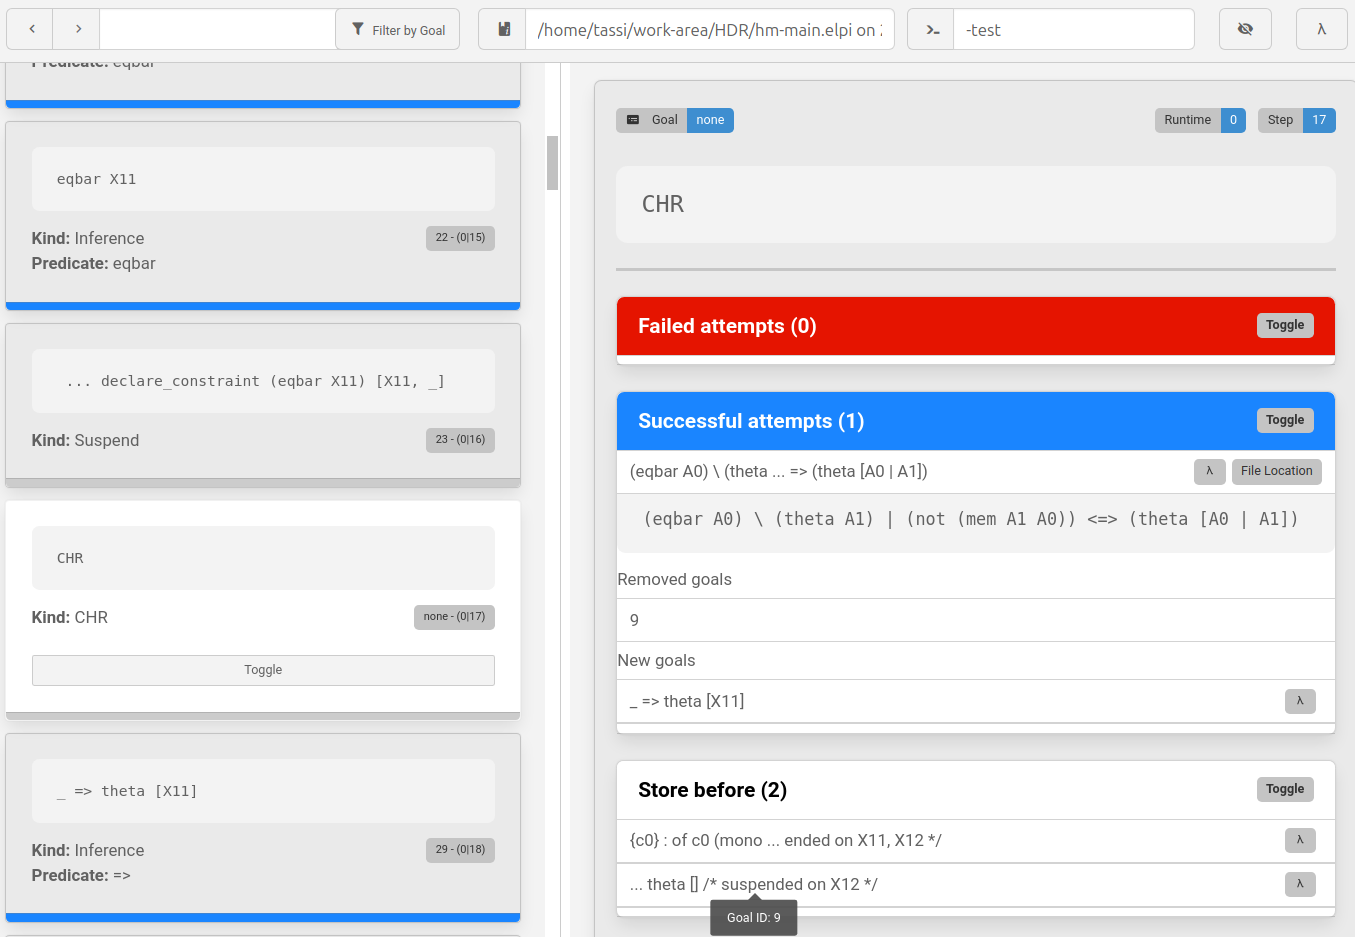
\includegraphics[width=.9\textwidth]{trace}

developed by Julien Wintz, it displays a trace as a mailbox of events
each events has pointers forward, backward and at a distance.
Each goal displays it full success or failure letting one
peek. The trace is searchable.

\chapter{Rocq-Elpi}\label{sec:rocq}

While Elpi is a standalone language and software project, it was designed to
play the role of an \emph{extension language} for Rocq. The glue between Elpi and
Rocq is called Rocq-Elpi.

My definition of this role, \emph{extension language}, is largely influenced
by the Lua programming language~\cite{10.5555/1200583}. Lua is an extension
language for applications written in C and is widely used in the Opens Source
world and in the gaming industry.
Its purpose is to provide an easy way to extend the host application.
It is easy to host Lua since its FFI is well curated, and thanks to that
exposing the internals of the application to the extension language requires a
limited effort to the application developer. It is easier to program in Lua,
rather than C, because the language is higher level, e.g. is features automatic
memory management and provides dictionaries as a builtin data structure.
Finally, it is easy for a user to get started with Lua because he does not need
to set up a proper development environment, the host application is sufficient
since Lua is an interpreter.\\
Elpi tries to do the same for OCaml, and Rocq is the host application of interest.

Even if we are not a big fan of it, in academia the same role is often called
meta-programming framework. Rocq's main data type, terms, are programs and Elpi
programs do manipulate Rocq programs. In this sense Elpi programs live at the
meta level.

\section{Why extending Rocq in OCaml is hard}

Luckily OCaml features automatic memory management, types and algebraic data.
It is much, much higher level than C. Why it is hard to extend Rocq then?

The first difficulty is that the complexity of the main Rocq data type, terms,
is not completely hidden by the algebraic data types provided by the programming
language. The missing features are encoded and it is hard to completely hide
it to the programer via curated APIs. In particular Rocq terms feature binders
and holes. 

Binders pose two problems of their own and interact badly with holes.
The first problem is that they are typically encoded with numbers, De Bruijn
indexes, and it is just too easy to forget to shift a term.  The second program
is that when a binder is crossed on must always remember something about it,
typically the type of the bound variable. Hence the programs have to pass around
typing contexts (aka environment). It is tempting to not do it upfront, but
expecting all developers, especially the casual ones, to be disciplined seems
a lost battle. We are in good company with this~\cite[page 20]{mcbride}:
``Mantra: $\Gamma$ is with me, wherever I go.''

Holes are missing subterms and they come with metadata: a typing sequent.
Since the same hole can occur non linearly a single sequent is stored on the side of terms.
Moreover since binders may be reduced away each occurrence has an explicit
substitution. So there is a state that accompanies the terms, a state to be
threaded in a functional setting. This state also gathers universe constraints,
as required by Rocq typical ambiguity (writing \rocq{Type} with no
explicit level).
Assignments are also part of this state and gives rise to weird concepts
like ``evar sensitive''. If one forgets to look at terms
through the right assignment (eg the empty one) the behavior is
hard to debug: it is like OCaml code that behaves differently depending
if a reference \ocaml{x} was originally given the value 42, of
if it was later updated to that value.
The example is not an exageration, this state is really like
a heap and if one has to manage it by hand it is like
going back to manual memory management, pointer dereferencing (with no
types), no gc.

The second difficulty is not inherent in OCaml, but rather an artifact of the
history of Rocq. The APIs are not well curated. Exposing some of them to
the extension language is a very good occasion to incrementally produce
a coherent set of APIs.

Last setting up the development environment and a development
process. Even when a user is past the, inevitablae, frustration
is setting up the right compiler and tools, an embedded
interpreter still gives some advantagess even more if the
language is rule based. One can iterate faster, without even
restarting the host application, and sometimes even modify
the code at a distance: even if the code is defined far away,
in a library being used, one can still replace bits of it code
here, where the problem shows up and conduct a must faster investigation.

\section{HOAS of Rocq terms and contexts}\label{GALLINA}

The main data type Rocq-Elpi programs work with is the one of
terms. The first bit of terms worth describing are the pointers
to global objects. While \elpi{constant}, 
\elpi{inductive} and \elpi{constructor} are opaque
data (as in \ref{sec:opaquedata}), their nature is exposed as
an algebraic data type.

\begin{elpicode}
kind gref type.
type const constant -> gref.            % Nat.add, List.append, ...
type indt  inductive -> gref.           % nat, list, ...
type indc  constructor -> gref.         % O, S, nil, cons, ...
\end{elpicode}

Global objects are injected in the term data type via the
\elpi{global} term constructor and its variant
\elpi{pglobal} dedicated to universe-polymorphic global
object.

\begin{elpicode}
kind term type.
type global  gref -> term.
type pglobal gref -> univ-instance -> term.
type sort    sort -> term.                 % Prop, Type@{i}, SProp
\end{elpicode}

We omit the algebraic data type for sorts and we rather focus on the
three binders: \elpi{fun} and \elpi{prod} for abstraction
and \elpi{let} for abbreviations.
Other than the higher order argument, the detail common
to all of the them is the \elpi{name} argument. It stands for
a pretty printing information, e.g. the bound variable as written by
the user. It is important to remark that \elpi{name} is
an opaque data type with a trivial euqality test. That is, the
name ``x'' and ``y'' are equal in Elpi, although they hold a
different value in OCaml. This is key to align the equational theory
of the meta language Elpi with a sensible notion of equality for
the object language Gallina, namely $\alpha$-equivalence.

\begin{elpicode}
type fun  name -> term -> (term -> term) -> term.            % λ
type prod name -> term -> (term -> term) -> term.            % ∀
type let  name -> term -> term -> (term -> term) -> term.    % let
\end{elpicode}

Application is n-ary, with the head and arguments hold by a list.
This choice, over binary application as in~\ref{sec:hello}, eases
the access to the head: according to our experience the vast majority
of rules is discriminated by the head constant of the terms they work on.

The pattern matching constructor packs together the scrutinee,
a term used to uniformly assign a type to branches and a list of
branches. The fixpoint operator is a binder, for the recursive call,
and carries the index of the decreasing argument. Finally a single
constructor holds all primitive values, eg 63 bit integers and floating
point numbers; primitive record projections.

\begin{elpicode}
type app       list term -> term.                     
type match     term -> term -> list term -> term.   
type fix       name -> int -> term -> (term -> term) -> term.
type primitive primitive-value -> term.
\end{elpicode}

What is worth focusing on is the representation of contexts, a convention
used when crossing binders to enable APIs to be called deep inside terms.
Two context entry need to be available, one for abstraction and one for
abbreviation.

\begin{elpicode}
pred decl i:term, o:name, o:term.                 % Var Name Ty
pred def  i:term, o:name, o:term, o:term.         % Var Name Ty Bo
\end{elpicode}

The first argument of each is, by convention, a bound variable, and is
expected to be passed as an input in order to retrieve the associaed
pretty pringing information, the type and in the case of
abbreviation the body. In the light of that code that crosses a binder
is expected to either declare a \elpi{decl} or a \elpi{def}
hypothetical rule for the bound variable as follows:

\begin{elpicode}
cross (fun N T F) :- pi x\ decl x N T => cross (F x).
\end{elpicode}

As a result of the convention, one can call \elpi{rocq.typecheck}
deep inside a term. As described in~\ref{sec:API} a predicate can
be equipped with a \ocaml{ctx_readback} function such
as \ocaml{proof_context} in the code below. The \ocaml{term}
contextual conversion can hence access a Rocq context when operating its
readback or embedding code.

\begin{ocamlcode}
MLCode(Pred("rocq.typecheck",
  CIn(term, "T",
  CInOut(B.ioargC term, "Ty",
  InOut(B.ioarg B.diagnostic, "Diagnostic",
  Full (proof_context, "typchecks a term T ...")))),
    (fun t ety diag _ proof_context _ state ->
      let sigma = get_sigma state in
      let sigma, ty = Typing.type_of proof_context.env sigma t in
      ...
\end{ocamlcode}

Indeed here the \ocaml{t} and \ocaml{ety} values
are read back in the \ocaml{proof_context.env} Rocq context,
that is also passed to the type checker in order to synthesize the
type of \ocaml{t}, and later (in the omitted code) to unify
the inferred type with the expected one \ocaml{ety} when provided.
The \ocaml{ioargC} lifts a contextual conversion to the option
type: if actual data is provided, then it is converted.

The only missing piece is \ocaml{sigma}, the environment assigning
type judgements to holes.

\section{HOAS of holes (missing terms)}

Each Rocq hole as an entry in \ocaml{sigma} that looks like a
typing sequent. In Elpi we represent it as a constraint \elpi{evar}.

\begin{elpicode}
pred declare-evar i:list prop, i:term, i:term, i:term. % Ctx RawEvar Ty Evar
declare-evar Ctx RawEv Ty Ev :-
  declare_constraint (declare-evar Ctx RawEv Ty Ev) [RawEv].

constraint declare-evar evar def decl {
  rule \ (declare-evar Ctx RawEv Ty Ev) <=> (Ctx => evar RawEv Ty Ev).
}
\end{elpicode}

Note how \elpi{declare-evar} uses the CHR meta level to craft
a goal with a precise context \elpi{Ctx}, no matter the context
under which \elpi{declare-evar} is generated. Ineed a Rocq API
that is called deep inside a term and that encounters a new hole has
will add to Rocq's sigma an entry for it, but also generate a
\elpi{declare-evar}, and hence an \elpi{evar} constraint
in Elpi.

The code above also relates a Rocq hole \elpi{Ev} and an
Elpi unification variable \elpi{RawEv}. We want the following
invariants to be hardwired on \elpi{Ctx => evar RawEv Ty Ev}.

\begin{itemize}
  \item \elpi{Ev} can only be assigned to a \elpi{R} if
        \elpi{R} has type \elpi{Ty} in context \elpi{Ctx}
  \item \elpi{RawEv} can only be assigned to a \elpi{X} if
        \elpi{X} elaborates to a term \elpi{R} such that
        the previous condition holds
\end{itemize}

The code below implements the desired invariants

\begin{elpicode}
pred evar i:term, i:term, o:term. % Evar Ty RefinedSolution
evar (uvar as X) Ty R :- declare_constraint (evar X Ty R) [X, R].
evar X Ty R :- not(var R), !, rocq.typecheck R Ty ok, X = R.
evar X Ty R :- not(var X), var R, !, rocq.elaborate-skeleton X Ty R ok.
\end{elpicode}

In the code above \elpi{rocq.elaborate-skeleton} is an API
very similar to \elpi{rocq.typecheck} but that does not modify
its input in place. It rather uses its input as a skeleton term that is
copied. This allows for changes to the structure of the term, like inserting
explicit coercions to implement type casts. The API corresponds to the code
that Rocq runs on any input term written by the user, while \elpi{rocq.typecheck}
corresponds to code internally used by Rocq tactics to build well typed terms.

The extensible state~\ref{sec:API} offered by Elpi carries a Rocq-Elpi specific
bidirectional map linked Rocq unification variables and Elpi holes.
It is built using this commodity Elpi API:

\begin{ocamlcode}
module FlexibleData : sig
  module Elpi : sig type t ... end
  module type Host = sig type t ... end
  module Map : functor(Host : Host) -> sig
    type t
    val empty : t
    val add : Elpi.t -> Host.t -> t -> t
    val elpi   : Host.t -> t -> Elpi.t
    val host : Elpi.t -> t -> Host.t
\end{ocamlcode}

TODO extra goals in API

TODO sigma in Elpi, sigma in Rocq, going from both.


%%%%%%%%%%%%%%%%%%%%%%%%%%%%%%%%%%%%%%%%%%%%%%%%%%%%%%%%%%%%%%%%%%%%%%%%%%%%%%%
%%%%%%%%%%%%%%%%%%%%%%%%%%%%%%%%%%%%%%%%%%%%%%%%%%%%%%%%%%%%%%%%%%%%%%%%%%%%%%%
%%%%%%%%%%%%%%%%%%%%%%%%%%%%%%%%%%%%%%%%%%%%%%%%%%%%%%%%%%%%%%%%%%%%%%%%%%%%%%


\section{Vernacular language integration}

That vernacular language of Rocq lets one organize the formalized knowledge,
in particular give names to Gallina terms and attach meta data to them.
Rocq-Elpi extends the vernacular language with a few commands to declare, run
and modify Elpi programs.

For convenience programs are divided into commands and tactics. Both run
Elpi code, but the entry point is different and moreover tactics can only
be executed in Rocq proof mode.

\subsection{Commands}

A command is declared with \rocq{Elpi Command} followed by a name.
Initially a command only contains the glue code for Rocq, like the
HOAS data type of terms and the builtin predicates. Extra code
can be added to a command via the \rocq{Elpi Accumulate}.
Accumulated code can have two natures: static code (e.g. from a file
or a string) and dynamic code (from a database, see~\ref{sec:homo}).

A command \texttt{hello} is executed with \rocq{Elpi hello} followed
by arguments. The \elpi{argument} data type has constructors
for builtin data type such as strings or number as well as Gallina terms.

\begin{rocqcode}
Elpi Command hello.
Elpi Accumulate hello lp:{{
  main [str X] :- rocq.say "Hello" X.
}}.
Elpi hello "reader".
Fail Elpi hello 46.
\end{rocqcode}

The simple program above calls the \elpi{rocq.say} builtin whenever the
command is passed a string. Since the entrypoint \elpi{main} has
no rule for arguments of the form \elpi{int X}.

The interested reader can look at the comprehensive tutorial on Elpi
commands~\cite{tuto:commands} that being part of the Rocq-Elpi software
distribution it is kept up to date.

\subsection{Tactics}

Tactics are built in a similar way, with the main difference being that
the entry point is called \elpi{solve} that receives as
argument not only the arguments passed to the tactic, but also the goal
on which the tactic operates.

\begin{rocqcode}
Elpi Tactic intro.
Elpi Accumulate intro lp:{{
  solve (goal _ _ _ _ [str ID] as G) GS :- !,
    std.assert! (rocq.ltac.id-free? ID G) "name already taken",
    rocq.id->name ID N,
    refine (fun N _ _) G GS.
}}.
Goal ∀P, P -> P /\ P.
elpi intro "p".
Fail elpi intro "p". (* Error: name already taken *)
elpi intro "Hp".
\end{rocqcode}

In the example above the tactic expects to receive a string \elpi{ID};
it checks that no Rocq proof variable is already using the same name, and
finally refines the goal with a lambda abstraction, that is the proof term
for logical rule of introduction of universal quantification or implication.
  
The interested reader can look at a longer tutorial on Elpi tactics~\cite{tuto:tactics}
and also to eltac~\cite{app:eltac}, a collection of Rocq tactics rewritten in Elpi for
didactic purpose.

\subsection{Databases, homoiconicity and rules}\label{sec:homo}

A database is, in its essence, an Elpi program but unlike commands and
tactics cannot be executed. It constitutes a pice of code that is
accumulated into commands or tactics \emph{by name}. This means that
whenever a program run its sees the current contents of the data bases
it accumulates, not their contents when the commands was inidially declared.

A typical data base is made of one predicate, possibly with some default
rules. The \rocq{Elpi Db} commands declares a data base.

\begin{rocqcode}
Elpi Db age.db lp:{{
  pred age o:string, o:int.

  % the Db is empty for now, we put a rule giving a
  % descriptive error and we name that rule "age.fail".
  :name "age.fail"
  age Name _ :- rocq.error "I don't know who" Name "is!".
}}.
\end{rocqcode}

Elpi rules can be given a name via the \elpi{:name} attribute.
Named rules serve as anchor-points for new rules when added to the Db.

A commands to print the age of a given name can be declred as follows

\begin{rocqcode}
Elpi Command age.
Elpi Accumulate Db age.db.
Elpi Accumulate lp:{{

  main [str Name] :-
    age Name A,
    rocq.say Name "is" A "years old".

}}.

Fail Elpi age bob. (* I don't know who bob is! *)
\end{rocqcode}

We can add entries to the data base manually as follows

\begin{rocqcode}
Elpi Accumulate age.db lp:{{

  :before "age.fail"     % we place this rule before the catch all
  age "bob" 24.

}}.

Elpi age bob. (* bob is 24 years old *)
\end{rocqcode}

We do not expect the users of Rocq commands written in Elpi to know the
syntax of Elpi, not the commands to manipulate its programs, and even more
to actually know the Rocq commands they run are implemented in Elpi.

For this reason Rocq-Elpi provides APIs to extend data bases from Elpi.
Here we craft a new command \rocq{set_age} that does use this API.

\begin{rocqcode}
Elpi Command set_age.
Elpi Accumulate Db age.db.
Elpi Accumulate lp:{{

  main [str Name, int Age] :-
    TheNewRule = age Name Age,
    rocq.elpi.accumulate _ "age.db"
      (clause _ (before "age.fail") TheNewRule).

}}.

Elpi set_age "alice" 21.
Elpi age "alice". (* alice is 21 years old *)
Elpi set_age "mallory" 24.
Elpi age "mallory". (* mallory is 24 years old *)
\end{rocqcode}

The same data bases can be accumulated by commands and tactics in order
to share a ``state'', a common knowledge that typically grows as the
commands or tactics are used in a Rocq library.

\subsubsection{Homoiconicity and rules}

There are two characteristic of Elpi that make data bases possible and also
handy to use.

The first one is that Elpi is a Homoiconic language: it can manipulate its own
syntax. The line

\begin{elpicode}
TheNewRule = age Name Age,
\end{elpicode}

is the simplest evidence of it: \elpi{TheNewRule} contains a pice
of Elpi code built from the \elpi{age} predicate and the two arguments
passed to \elpi{main}. Since construction/inspection are conflated
into unification in logic programming, the same line can be used to analyze the
syntax of a piece of code in order to extra the name and age.

The second characteristic of Elpi that really helps is that the code is
organized into rules, meaning that \elpi{age Name Age} is an entire code
unit one can build or inspect. In comparison the OCaml code for the
\ocaml{age} function is a single expression (a single unit):

\begin{ocamlcode}
let age s =
  match s with
  | ("bob" | "mallory") => 24
  | "alice" => 21
  | _ => failwith ("I don't know who " ^ s ^ " is!")
\end{ocamlcode}

While it is surely possibe to traverse the syntax tree above and add one
pattern match branch before the last one, that manipulation is not completely
trivial. To make it so one should opt out of most of the syntactic sugar and
commit to use a syntactic form that is as close as possible to the one
of a rule based language:
\begin{itemize}
  \item making all variable bindings local to the pattern matching branch branch
  \item making all rules syntactically independent
\end{itemize}

The code below respects these points. Remak \ocaml{s} binding now
being local to the last branch, and the separation between the bob and
mallory branches:

\begin{ocamlcode}
let age = function
  | "bob" => 24
  | "alice" => 21
  | "mallory" => 24
  | s => failwith ("I don't know who " ^ s ^ " is!")
\end{ocamlcode}
  
The syntactic price one pays when writing Elpi code is now partially
compensated by the ease of extending existing code.
The example in the following section makes good use of this possiblity.

\section{Example: simple proof transfer}\label{sec:tb}

We provide an example of a tactic and a command that communicate via
a database. The tactic \rocq{to_bool} transfers a goal from the realm
of propositions to the one of computable (boolean) tests (decidable propositions).
The command \rocq{register_decision} takes a proof of equivalence
between a proposition and a boolean test and ``compiles'' it to an Elpi rule.
The database contains all the known rules for translating propositions into
tests: it is queried by \rocq{to_bool} and populated by \rocq{register_decision}.

It is customary to organize Rocq-Elpi code in this very way. The key feature
one obtains is that the \rocq{to_bool} is extensible: when a new
predicate is declared and a new test defined, it is sufficient to call
\rocq{register_decision} to extend \rocq{to_bool} with the new
predicate.

We assume a Rocq environment with the following lemmas. The \rocq{reflect}
predicate links a proposition with a boolean test: \rocq{reflect P b}
means \rocq{P} holds if and only if \rocq{b = true}.

\begin{rocqcode}
Lemma evenP n : reflect (is_even n) (even n).

Lemma andP  {P Q : Prop} {p q : bool} :
  reflect P p -> reflect Q q -> reflect (P /\ Q) (p && q).

Lemma elimT {P b} :
  reflect P b -> b = true -> P.
\end{rocqcode}

The database holds rules for the \elpi{tb} relation. Since
we are only interested in one direction of the equivalence we
relate a proposition with its equivalence proof (disregarding the
associated boolean test).

\begin{rocqcode}
Elpi Db tb.db lp:{{

% [tb P R] finds [R : reflect P b] for some b
pred tb i:term, o:term.

:name "tb:fail"
tb Ty _ :- rocq.error "Cannot solve" {rocq.term->string Ty}.

}}.
\end{rocqcode}

The database only contains one rule aborting the search with an error message.
All rules will need to be placed before that one.

The \rocq{to_bool} tactic is built as follows a top of the
database.

\begin{rocqcode}
Elpi Tactic to_bool.
Elpi Accumulate Db tb.db.
Elpi Accumulate lp:{{

solve (goal Ctx _ Ty _ _ as G) [G1] :-
  tb Ty P,
  refine {{ elimT lp:P _ }} G [G1].

}}.
\end{rocqcode}

The tactic simply queries the database for a proof \elpi{P} that
the goal is related to a boolean test, then refines the goal (as in the
standard Rocq \rocq{refine} tactic) with \rocq{elimT lp:P _}.
The hole stands for the proof of \rocq{b = true}, i.e. the subgoal
\elpi{G1}.

The most interesting part of this example is how the dabase is populated.
We shall write a \elpi{compile} procedute that given \rocq{evenP}
and \rocq{andP} synthesizes the following Elpi code

\begin{elpicode}
tb {{ is_even lp:N }} {{ evenP lp:N }} :- !.
tb {{ lp:P /\ lp:Q }} {{ andP lp:PP lp:QQ }} :- !, tb P PP, tb Q QQ.
\end{elpicode}

As sketched in~\ref{sec:homo}, the two rules above corrspond to the
following (closed) Elpi terms:

\begin{elpicode}
pi N\ tb {{ is_even lp:N }} {{ evenP lp:N }} :- [!]
pi P Q PP QQ\ tb {{ lp:P /\ lp:Q }} {{ andP lp:PP lp:QQ }} :-
  [!, tb P PP, tb Q QQ].
\end{elpicode}

It is worth unfolding quotations to see that a few more quantifications are
necessary for the second rule

\begin{elpicode}
pi P Q p q PP QQ\
  tb (app[global (indt "/\"), P, Q])
     (app[global (con "andP"), P, Q, p, q, PP, QQ]) :-
  [!, tb P PP, tb Q QQ].
\end{elpicode}
  

Now that all quantifications are explicit we can look at the types of
\rocq{evenP} and \rocq{andP} and remark how each \elpi{pi}
Elpi quantification corresponds to a Rocq quantification (dependent or not),
and Rocq premises corresponds to recursive calls in Elpi.

\begin{rocqcode}
evenP : ∀n, reflect (is_even n) (even N).
andP : ∀P Q p q,
  reflect P p -> reflect Q q -> reflect (P /\ Q) (p && q).
\end{rocqcode}

The \elpi{compile} predicate has three inputs an one output.
The first input is the type of a lemma and the second is the proof of that
lemma, this relation between the first two argument is a key invariant.
The third argument is a list of recursive calls, while the output is
the code of the Elpi rule being generated.

\begin{elpicode}
pred compile i:term, i:term, i:list prop, o:prop.

compile {{ reflect lp:Ty _ }} P Hyps (tb Ty P :- [! | Hyps]).

compile {{ reflect lp:S _ -> lp:T }} P Hyps (pi h\ C h) :- !,
  pi h\ compile T {{ lp:P lp:h }} [tb S h | Hyps] (C h).

compile {{ ∀x, lp:(T x) }} P Hyps (pi h\ C h) :-
  pi x\ compile (T x) {{ lp:P lp:x }} Hyps (C x).
\end{elpicode}

The first rule is the base case. When we reach the conclusion of the lemma
\rocq{reflect lp:Ty _} we know that the second argument \elpi{P}
is a proof of that fact, hence \elpi{tb Ty P} is a correct head for the
rule. The premises of the rules are the \elpi{Hyps} recursive calls
prefixed with a cut.

The second rule is for premises that are turned into recursive calls. In this
case the output rule features an extra \elpi{pi} quantification and the
\elpi{Hyps} list gets longer. The \elpi{h} variable stands for
the proof obtained by the recursive call, a proof of \rocq{reflect lp:S _}
hene an argument we can pass to the second argument as in \rocq{lp:P lp:h}
so to keep the invariant that it is a proof of \elpi{T}, the type
in which we recurse.

The last rule is a simpler version of the second, in this case the quantification
is not a premise, hence we do not extend \elpi{Hyps}.

The code of the \rocq{register_decision} command located the
given lemma, finds its type and generates the new rule \elpi{C}.
finally it adds the rule to the database before the \elpi{"tb:fail"}
anchor point.

\begin{rocqcode}
Elpi Command register_decision.
Elpi Accumulate Db tb.db.
Elpi Accumulate lp:{{
    
main [str S] :-
  rocq.locate S GR,
  rocq.env.typeof GR Ty,
  compile Ty (global GR) [] C,
  rocq.elpi.accumulate _ "tb.db" (clause _ (before "tb:fail") C).

}}.
\end{rocqcode}

We can now populate the database and test our tactic.

\begin{rocqcode}
Elpi register_decision andP.

Lemma test : is_even 6 /\ is_even 4.
Proof.
elpi to_bool. (* Error: Cannot solve is_even 6 *)
Abort.

Elpi register_decision evenP.

Lemma test : is_even 6 /\ is_even 4.
Proof.
elpi to_bool. (* even 6 && even 4 = true *)
simpl.        (* true = true *)
trivial.
Qed.
\end{rocqcode}
  
The Rocq snippet calls the \rocq{to_bool} tactic in a scenario
where a predicate is not (yet) registered obtaining an explicative
error message. Then it register a test for the missing predicate
and succesfully solves the goal.


\chapter{Rocq tools written in Elpi}

In this chapter we survey some tools developed on top of Rocq-Elpi.
We put forward Derive and Hierarchy Builder, to which we contributed personally.
Last we quickly survey other tools developed by our colleagues.

At the end of each section we discuss which features of Elpi and Rocq-Elpi
are key to the tool being described.

\section{Derive}\label{sec:derive}

The derive application is a framework for automatic
code generation, typically in response to the declaration of a new inductive
data type.

Rocq itself is known to generate induction principles and equality tests.
Unfortunately it is also known to generate bad induction principles when
containers (e.g. lists) are involved and often fail to generate useful
equality tests.

We saw the opportunity to improve on that starting with the L3 internship of
Luc Chabassier that wrote the first prototype in the summer of 2017.
He succeeded in generating
equality tests and their proofs in two months. While most of the credit goes to
his learning skills, the experience confirmed that Rocq-Elpi was able to support
research in this domain. Indeed the solution implemented by Luc, although
correct, was not very satisfactory since it was not modular. Improving
on that lead to~\cite{tassi:hal-01897468} that describes a skema to
generate so called deep induction principles and uses them to prove
equality tests correct. Before discussing that work we need to introduce
the swiss army knife of boilerplate code generation: parametricity.

\subsection{Parametricity}\label{sec:param1}

The so called parametricy translation \cite{keller_et_al:LIPIcs.CSL.2012.381}
is a family of procedures $[\cdot]_i$ indexed by an arity $i$. We focus on the
unary one, i.e. $i=1$, and we write $U$ for any Rocq universe, i.e. \rocq{Prop}.
Given \emph{any} Rocq term $t : r$, the unary parametricity
translation gives both a unary predicate $R$ on $r$, e.g. $[r]_1 = R : r \to U$
and a proof $T$ that $R$ holds for $t$, i.e. $[t]_1 = T : R~ t$ or somewhat more
confusingly if $t : r$ then $[t]_1 : [r]_1~ t$.

For example the unary parametricity translation of
\rocq{nat} is \rocq{is_nat : nat → U} and
the translation of \rocq{3 : nat} is a proof that \rocq{is_nat 3}.

\begin{rocqcode}
Inductive is_nat : nat -> U :=
| is_zero : is_nat 0
| is_succ n : is_nat n -> is_nat (S n).

Definition is_nat_3 : is_nat 3 :=
  is_succ 2 (is_succ 1 (is_succ 0 is_zero)).
\end{rocqcode}

One can see \elpi{is_nat} as a first class description of the
typing assignment, i.e. each term is equipped with a proof that
is has the expected type, i.e. \rocq{0} with \rocq{is_zero};
\rocq{1} with \rocq{is_succ 0 is_zero}, and so on.

The translation becomes interesting when the type has parameters such as
\rocq{A} in \rocq{list A}. In that case the translation builds
a predicate parametric in \rocq{A} and in its translation. For example
the translation of \rocq{list A} is a predicate
\rocq{is_list : ∀A, (A → U) → (list A → U)},
and the translation of the constructors \rocq{nil} and \rocq{cons}
are:
\begin{rocqcode}
is_nil: ∀A (isA : A → U), is_list A isA nil
is_cons: ∀A (isA : A → U), ∀a, isA a → 
  ∀l, is_list A isA l → is_list A isA (a :: l).
\end{rocqcode}

As for the translation of natural numbers, each term comes with a proof
that is has the expected type. When the term is of type \rocq{A},
the type parameter of the container, then it comes with a proof of \rocq{isA},
the predicate parameter associated with \rocq{A}.
The unary parametricity translation is the key to express, in a
systematic way, that a property holds deep inside a container.

The parametricity translation is a meta program in Rocq, it cannot be implemented in
Gallina itself hence one needs a meta language to implement it.
Cyril Cohen implemented the binary parametricity translaton in the fall of 2017,
as he was interested in employing the translation in the Rocq-EAL project.
We based the unary version on his code. Each translation is about 250 lines
of Elpi code.

\subsection{Deep induction}

We say that an induction principle is deep if the induction hypothesis is
available for sub terms that occur deep inside the immediate sub terms.
As an example we can take the data type of rose trees.

\begin{rocqcode}
Inductive rtree A : U :=
| Leaf (a : A)
| Node (l : list (rtree A)).
\end{rocqcode}

The induction principle generated by Rocq is shallow: \rocq{P} is
only available on the immediate subterms of type \rocq{rtree}, that
in this case are none.

\begin{rocqcode}
Lemma rtree_ind : ∀A (P : rtree A → U),
  (∀a : A, P (Leaf A a)) →
  (∀l : list (rtree A), P (Node A l)) →
  ∀t : rtree A, P t.
\end{rocqcode}

That principle is weak since no element of \rocq{l} in \rocq{Node A l}
verifies \rocq{P}. In \cite{tassi:hal-01897468} we study the synthesis
for a stronger principle where \rocq{P} holds deep inside \rocq{l}.

\begin{rocqcode}
Lemma rtree_induction A is_A (P : rtree A → U) :
  (∀a, is_A a → P (Leaf A a)) →
  (∀l, is_list (rtree A) P l → P (Node A l)) →
     ∀t, is_rtree A is_A t → P t.
\end{rocqcode}

The induction principle uses the unary parametricty
translation of \rocq{l} and its type in order to systematically craft
the hypothesis \rocq{is_list (rtree A) P l} that gives access to
\rocq{P} on all elements of \rocq{l}.

This  extra assumption comes at a price: the induction principle does not apply
to to just a tree, but to a tree \elpi{t} such that
\rocq{is_rtree A is_A t} holds. This extra argument is
synthesized automatically.

For non-containers like \rocq{nat}
we prove \rocq{∀n, is_nat n} by induction on \rocq{n} (no different
than how we proved \rocq{is_nat 3} before). For containers we prove
the statement under the assumption that the predicate for the type parameter
is triviall true. E.g.

\begin{rocqcode}
Lemma list_is_list A isA : (∀a, isA a) -> ∀l, is_list A isA l.
Lemma rtree_is_rtree A isA : (∀a, isA a) -> ∀l, is_rtree A isA l.
\end{rocqcode}

While the assumption seems strong at first, it actually matches two relevant class
of predicates:
\begin{itemize}
  \item the one we are definig, e.g. \rocq{nat_is_nat} fits
  \item any \rocq{P : t -> U} we are defining by induction on the whole
    type \rocq{t}, e.g. the \rocq{P} of an induction principle
\end{itemize}

In order to prove the deep induction principle we need some scaffolding,
again synthesized automatically via Elpi programs. The first one
allows us to operate under a unary parametricity translation.

\begin{rocqcode}
Definition is_list_functor A P Q :
  (∀a, P a → Q a) → ∀l, is_list A P l → is_list A Q l
:=
  λ(f : ∀a, P a -> Q a) =>
    fix IH l (pl : is_list A P l) {struct pl} : is_list A Q l :=
      match pl in (is_list _ _ s1) return (is_list A Q s1) with
      | is_Nil _ _ => is_Nil l pl
      | is_Cons _ _ a Pa xs Pxs =>
          is_Cons A Q a (f a Pa) xs (IH xs Pxs)
      end
\end{rocqcode}

The proof is a straightforward induction on list \rocq{l}.
We can now present the proof of the deep induction principle over rose trees:

\begin{rocqcode}
Definition rtree_induction (A : U) (PA : A → U) (P : rtree A → U)
    (His_Leaf : ∀a, PA a → P (Leaf A a))
    (His_Node : ∀l, is_list (rtree A) P l → P (Node A l))
:=
  fix IH s1 (x : is_rtree A PA s1) {struct x} : P s1 :=
  match x in (is_rtree _ _ s2) return (P s2) with
  | is_Leaf _ _ a Pa =>
      His_Leaf a Pa
  | is_Node _ _ l Pl =>
      His_Node l (is_list_functor (rtree A) (is_rtree A PA) P IH l Pl)
  end.
\end{rocqcode}

Remark the following type assignments for the variabls and terms occurring
in the last branch of the \rocq{match} on \rocq{x}:

\begin{rocqcode}
l  : list (rtree A)
Pl : is_list (rtree A) (is_rtree A PA) l
IH : ∀r, is_rtree A PA r -> P r
is_list_functor (rtree A) (is_rtree A PA) P IH l Pl :
  is_list (rtree A) P l
\end{rocqcode}

The last term satisfies the premise of \rocq{His_Node}, that in turn
gives the user of the induction principle access to the property \rocq{P}
on all the elements of \rocq{l}.

\subsection{Natural equality tests}

Now that we have a good induction principle we can prove the following
properties about the recursive program of interest.

\begin{rocqcode}
Definition correct (T : Type) (eqb : T -> T -> bool) :=
  ∀x y : T, reflect (x = y) (eqb x y).

Definition correct_at (T : Type) (eqb : T -> T -> bool) (x : T) :=
  ∀y : T, reflect (x = y) (eqb x y).
\end{rocqcode}

This is the form of correctness lemmas we shall prove.

\begin{rocqcode}
Lemma seq_eq_correct : ∀A eqA (l : list A),
  is_list A (correct_at A eqA) l ->
    correct_at (list A) (list_eq A eqA) l
\end{rocqcode}

It reads: if \rocq{eqA} is a correct test on all elements of \rocq{l},
then \rocq{list_eq A eqA} is a good test for \rocq{l}.

The interesting case the the equality test for rose trees, that reuses
the equality test for lists \rocq{list_eq} passing the recursive call
at the \rocq{eqA} argument.

\begin{rocqcode}
Definition rtree_eq A (A_eq : A → A → bool) :=
  fix rec (t1 t2 : rtree A) {struct t1} : bool :=
    match t1, t2 with
    | Leaf a, Leaf b => A_eq a b
    | Node l, Node s => list_eq (rtree A) rec l s
    | _, _ => false
    end.
\end{rocqcode}

What is remarkable is that the correctness proof for \rocq{rtree_eq}
reuses the correctness proof for \rocq{list_eq}.

\begin{rocqcode}
Definition rtree_eq_correct (A : Type) (eqA : A -> A -> bool) :
  ∀r, is_rtree A (correct_at A eqA) r ->
        correct_at (rtree A) (rtree_eq A eqA) r
:=
  rtree_induction
    A (correct_at A eqA) (correct_at (rtree A) (rtree_eq A eqA))
    (λ(a0 : A) (Pa : correct_at A eqA a0) =>
       correct_Leaf A eqA a0 Pa)
    (λ(sib : list (rtree A))
         (Psib : is_list (rtree A)
                   (correct_at (rtree A) (rtree_eq A eqA)) sib) =>
       correct_Node A eqA sib
         (list_eq_correct (rtree A) (rtree_eq A eqA) sib Psib)).
\end{rocqcode}

The proof also uses two auxiliary lemmas that are not particularly interesting,
we point the reader to~\cite{tassi:hal-01897468} for details about them.

\begin{rocqcode}
correct_Node : ∀A eqA (l : list (rose A)),
  correct_at (list (rose A)) (list_eq (rose A) (rose_eq A eqA)) l ->
    correct_at (rose A) (rose_eq A eqA) (Node A l)

correct_Leaf : ∀A eqA (a : A),
  correct_at A eqA x ->
    correct_at (rose A) (rose_eq A eqA) (Leaf A x)
  \end{rocqcode}
  
The final theorem can be obtained by satisfying the extra the extra
premise of the deep induction hypothesis, namely that each rose tree
is a rose tree.

\begin{rocqcode}
Definition rose_eq_OK A eqA :
  correct A eqA -> correct (rtree A) (rose_eq A eqA)
:=
  λp r =>
    rose_eq_correct A eqA
      r (rtree_is_rtree A (correct_at A eqA) p r).
\end{rocqcode}

To conlude, both euqality tests and their proofs are built compositionally.
In~\cite{tassi:hal-01897468} we also discuss why these proofs can be kept opaque
without interfeering with the termination checker.

\subsection{Fast equality tests}

The results in~\cite{tassi:hal-01897468} are futher refined in~\cite{gregoire:hal-03800154}
where we focus on the size (and hence type checking time) of the terms
synthesized. In particular the natural equality tests are quadratic: they
compare each constructor with all the others. Consequently proofs are also
quadratic in the number of constructors.

In~\cite{gregoire:hal-03800154} we devise equality tests that are pseudo
linear in size and we prove them correct in a compositional way using the deep
induction principles devised in~\cite{tassi:hal-01897468}.

We sketch here only the pseudo linear skema for rose trees. The idea
is to assign to each constructor a tag (a positive number) and
compare these tags upfront. If the tags are different then
the two rose trees are different, while if they are equal we can
uniformly unpack the fields and compare them.

We synthesize upfront these three functions.

\begin{rocqcode}
Definition tag A : rtree A -> positive.
Definition fields_t : positive -> Type.
Definition fields A :  ∀r : rtree A, fields_t (tag t).
\end{rocqcode}

The main code mattern matches over the first \rocq{rtree} and 
pre-computes its tag and fields. The it calls a common piece of
code \rocq{eqb_body} that will test if the tags agree and proceed
if it is the case.

\begin{rocqcode}
Definition rose_eqb A eqA : rtree A -> rtree A -> bool := 
  fix rec (x1 x2 : rose A) {struct x1} : bool :=
    match x1 with
    | Leaf _ a =>
        (* 1 = tag (Leaf _ a); a = fields (Leaf _ a) *)
        eqb_body 1 (eqb_fields A eqA rec) a x2
    | Node _ sib =>            
        (* 2 = tag (Node _ sib); sib = fields (Node _ sib) *)
        eqb_body 2 (eqb_fields A eqA rec) sib x2
    end.
\end{rocqcode}

When the tags agree, \rocq{eqb_body} extracts the fields
of the second rose tree and calls \rocq{eqb_fields}.
Since the two fields have, respectively, type 
\rocq{fields_t t1} and \rocq{fields_t t2} a cast is necessary.

\begin{rocqcode}
Definition eqb_body t1 eqb_fields v1 x2 :=
  let t2 := tag x2 in
  match pos_eq_dec t2 t1 with
  | left heq =>
    let f2 : fields_t t2 := fields x2 in
    eqb_fields t1 f1 (match heq with eq_refl => f2 end)
  | right _ => false
  end.
\end{rocqcode}

Comparing the fieds amounts at calling the equality test for the
right type, possibly using the recursive call to \rocq{rose_eqb}.

\begin{rocqcode}
Definition eqb_fields A eqA rec t :
  fields_t t -> fields_t t -> bool
:=
  match t as i return (fields_t i -> fields_t i -> bool) with
  | 1%positive => λa b : A => eqA a b
  | 2%positive => λa b : list (rtree A) =>
                    list_eqb (rtree A) rec a b
  | _ => λ_ _ => true (* impossible, only 2 constructors *)
\end{rocqcode}

As we can see the two matches of the constructors are no nested, but rather
chained. Both \rocq{rose_eqb} and \rocq{eqb_fields} have a number
of branches proportional to the number of constructors.

The main downside is that, unless the quality tests gets extracted to
OCaml, the type cast that uses the evidence provided by \rocq{pos_eq_dec}
has to be evaluated. The reader interested in benchmarks
can find them in~\cite{gregoire:hal-03800154}.

\subsection{The role of Rocq-Elpi in derive}
The Elpi language turned out to be instrumental in this research since
it allowed to quickly and concisely write derivations. We believe that
the automatic handling of names and holes was key. Only a few Rocq APIs were
really necessary: reading from and writing to the logical environment and
invoke type inference. Although these API come with glue code that is far from
trivial since they read/write inductive types in HOAS form.
Performance was no crytical: all bottlenecks turned out to be inefficiencies
in Rocq, and in particular in the APIs to manage universe constraints.


\section{Hierarchy Builder}\label{sec:hb}

The Mathmatical Components library is the largest an most widely used
mathematical library for Rocq according to the 2022 Rocq users
survey~\cite{dealmeidaborges_et_al:LIPIcs.ITP.2023.12}.
It is the pillar that was built for
tackling the mechanization of the Odd Order theorem~\cite{DBLP:conf/itp/GonthierAABCGRMOBPRSTT13}.
A key ingredient of this pillar is the hierarchy of interfaces around which
the contents are orgnized and the fine tuning of the mechanisms that
link the interfaces to their instances: the elaborator of Rocq is
programmed to automatically find a justification when an abstract theory
is applicable to an instance.

The Achilles'heel of the library is the barrier to entry, and while
documentation as in \cite{assia_mahboubi_2022_7118596} surely helps,
the complexity of building the hierarchy and programming the elaborator
could not be tamed by just explaining, exacly as assembly cannot be made
amenable by just documenting it. Hierarchy Builder (HB) provides a high level,
declarative language to describe the hierarchy and a ``compiler'' that
translate this language down the foundational language of Rocq and takes
care of programming the elaborator to make the hierarchy work.

The design of the language was brought to our attention in Spring 2019
by Cohen Cyril, the result of fruitful discussions with other
researchers in this domain in a Dagstuhl seminar. The implementation
took six months~\cite{cohen_et_al:LIPIcs.FSCD.2020.34} and pushed
Rocq-Elpi to bind a large set of Rocq APIs. The ``boilerplate'' code
HB substitute with a metaprogram has to declare Rocq modules, sections,
notations, implicit arguments, canonical structures \ldots in addition
to records and functions between records. HB also motivated the possibility
to pass Rocq-Elpi programs arguments that are Rocq declarations, such as the ones intruced by
the \rocq{Record} or \rocq{Definition} keywords.


\subsection{Mathematical Components 2.0 and M.C.A.}

Even if HB was, in principle, capable to describe all the interfaces of
the Mathematical Components library, it was still a huge effort to port the
library to the HB language.  We were lucky that developers and power users of
Mathematical Components agreed to work on it during a week-long coding
sprint~\cite{affeldt:hal-03463762}. The results surpassed our expectations:
not only the library was ported, but many satellite projects moved to
HB as well.

The ease in defining new interfaces brought by HB unlocked 
the growth of the mathematical components library, in particular of
its order theory component. The graph in Figure~\ref{fig:mc} shows in green the
number of interfaces defined using HB.

\begin{figure}[!ht]
\includegraphics[width=\textwidth,trim={2cm 4cm 2cm 4cm},clip]{hb\_intf.pdf}
\caption{Evolution of the Mathematical Components library\label{fig:mc}}
\end{figure}

One can see that since HB was introduced the number of
interfaces started to grow steadily. In the last three years about a hundred
of them were added, almost doubling their overall quantity,
while in the previous zeven years only a handful.
One can also see that the size of the library shrunk visibly as the result of
the porting, since the HB language hides boilerplaec code that has a size
(when hand written) quadratic in the number of related interfaces.

We want to stress the link between the growth of the hierarchy of interfaces and
the growth of the actual contents (definitions and theorems) of a formal
library. Figure~\ref{fig:mca} shows the steady progress made by the
Mathematical Components Analysis library (MCA).

\begin{figure}[!hb]
\includegraphics[width=\textwidth,trim={2cm 4cm 2cm 4cm},clip]{hb\_intfa.pdf}
\caption{Evolution of the Mathematical Components Analysis library\label{fig:mca}}
\end{figure}

The developmers of MCA adopted HB even before MC was ported to it, roughly from
the very beginning of the library development. The graph testifies how
the growth of a that library went hand in hand with the growth of
its hierarchy of interfaces. Something similar can also be observed in
\ref{fig:mc} although before the advent of HB the addition of an interface
was requiring the addition of very large boilerplate code, somewhat forcing
the correlation between the two measures: the port to HB resulted in the
removal of 5K lines of such boilerplate code.

\subsection{The role of Rocq-Elpi in Hierarchy Builder}

During the first implementation of HB, version 1.0, Elpi as a language was
really a technical advantage: its high level nature let us quickly experiment
with different solutions. Once the design was finalize, we thought that rewriting
the tool in OCaml, if necessary, would be possible. Then HB had to be substantially
changed in order to accommodate for interfaces with parameters, with the objective
to really apply it to the Mathematical Components library. This huge rewriting
turned out to possible since Elpi featured a type checker and that the change
could be modelled as a data type change: the description of an interface moved from
a flat list to a HOAS one, describing how formal (bound) parameters distribute over
the sub interfaces. A posteriori we think we could have done the same
refactoring to an OCaml program, but while it was natural to move to HOAS
in Elpi, it is unclear if the right reflex would have emerged in OCaml where
binding is not necessary reflected in the types.

The development and use in production of HB unraveled a few inefficiencies
in the implementation of HB and Elpi. Luckily they were mostly due to
a few very naive routines, in terms of computational complexity.

All the inefficiencies in HB can be imputed to the skinny standard library
of Elpi. For example, a hierarchy is essentially a Directed Acyclic Graph that
describes an order relation. Topologically sorting a sub part of it is a
frequent operation in HB and our first naive implementation was cubic.
Similarly, when we see hierarchy nodes as designated sets and
edges as the superset relation, we often need to find all the designated
sets included in a given one. An algorith properly exploiting the DAG
can discard all the supersets of any set that is not included in the given one,
while a naive algorithm can only filter the designated sets, linearly.

More surprisingly the inefficiencies found in Elpi were not in the runtime
of the language, but rather in its compiler, and more specifically in
its (lack of) incrementality. As exemplified in~\ref{sec:tb}, HB synthesizes
and accumulates rules as it goes to represent its state. In MC alone
the number of such rules reaches 40K, and any routine that was not incremental
and/or had a bad complexity had to be revised. In particular the version 2.0 of
Elpi has a fully incremental compiler: adding a rule to an existing program (or
data base) has logaritmic complexity in the size of the interested
part of program, i.e. the existing rules for the same predicate.

To the best of our knowledge, today most of the time spent in HB is actually taken
by calls to Rocq API, typically to typecheck and define the terms that are
automatically synthesized.

\section{Other tools}

Rocq-Elpi found applications in other projects we did not participate
into directly. Here we mention some we are aware of.

\subsection{Algebra Tactics}

Algebra tactics is a port (and improvement) of the \rocq{ring}, \rocq{field} and
\rocq{lra} tactics to the Mathematical Components library~\cite{sakaguchi:LIPIcs.ITP.2022.29}.
These tactics are reflexive, i.e. a pre-processing phase called reification
recognizes in a goal the syntax of an algebraic structure and reflects it into
a datatypes that is then manipulated by a certified Gallina program.
Given the hierarchy of structures, operations typical of a structure may be
inherited from a substructure. Since the type theory of Rocq does not feature
subtyping, the cast of a structure to a substructure leaves a trace in
the terms of Gallina, making the reification work more delicate.

For example the addition of a ring actually comes from the
additive abelian group it inherits from. The code snippet below
has to compare the abelian group instance \elpi{U} with the ring
instance \elpi{R} the tactic is applied to, possibly in the context
\elpi{C} of a ring morphism.

\begin{elpicode}
ring C {{ @GRing.opp lp:U lp:In1 }} {{ @ROpp lp:R lp:OutM1 }} Out VM :-
  rocq.unify-eq { rmorphism->zmod C } U ok,
  rmorphism->ring C R, !,
  ring C In1 OutM1 Out1 VM, !,
  build.opp Out1 Out.  
\end{elpicode}

\subsubsection{The role of Rocq-Elpi in Algebra Tactics}

The code crytically uses the possibility to call
the \elpi{rocq.unify-eq} deep inside the goal to identify
terms up to (Rocq) unification.

The algrbra tactics project comprises a few benchmarks including
a five hundred lines long polynomial euqation in six variables.
The \rocq{ring} tactic takes about five seconds to solve it.

While the standard, simpler, reification writtne in OCaml is an order of
magnitude faster, the reification procedure written in Elpi is not the dominant
factor in the five seconds, making it usable, in practice, even on such an
extreme goal (for an interactive theorem prover).


\subsection{Takt and TRocq: proof transfer tools}

The most frequently asked question regarding the Mathematical Components
library is: how do we make it compute.

Almost all definitions in the MC library
are computable, but are not immediately executable by Rocq for one of
the following two reasons. Either they are executable but are inefficient
being optimized for proofs and not computations, or they are ``locked''
behind an opaque module signature to enforce an abstraction barrier previnting
the Rocq type checker to potentially take an unreasonable amount of time.

The answer to the FAQ is to transfer an expression about inefficient or
locked operations to (equivalent) fast and unlocked ones. While defining
such operations and proving the correspondence is feasible, and sometimes
even part of the MC library, the tooling to automatically perform
the transfer never really existed in a easy to use form.

The Trakt tool~\cite{DBLP:conf/cpp/Blot0CPKMV23} and its successor
Trocq~\cite{10.1007/978-3-031-57262-3_10} fill this space. Both
are implemented in Elpi and are organized as sketched in~\ref{sec:tb}.
Trocq is based on a gradualized version of the Univalent Parametricity
translation~\cite{10.1145/3429979}. Unlike the parametricity relation
sketched in~\ref{sec:param1} that talks about bare bone relations, the univalent
version focuses on relations that are equivalences.
Trocq improves on that by studying the relations that are in between,
like implication (i.e. type theoretic maps).
It turns out that in many cases of practical interest the type
theory of Rocq, that does not internalize the principle of univalence, is
sufficient to represent the result of the parametricy translation
for non bare-bone relations.

\subsubsection{The role of Rocq-Elpi in Trocq}

In his PhD disseration~\cite[Page 115]{enzo}, Crance
highlights how naturally pen-and-paper Trocq rules can be transposed in Elpi.
It is worth mentioning that Crance uses Constraints Handling Rules to
store axiom-requirements when translating an expression, and only when
all requirements are know he computes the minimum set of Rocq axioms
needed in order to represent the parametricity based translation.

% \subsection{EIris: ???}

% https://github.com/lukovdm/MasterThesisIrisElpi/blob/e7c9f2a835a523fa8937b24f06bac061e5f50ab9/latex/thesis/thesis.pdf

\subsection{BlueRock's BRiCk}

BlueRock systems is a company developing, among other things, the BRiCk
program logic for C++. It is a set of Rocq libraries, partially based on Iris,
to reason about existing C++ code: a \texttt{cpp2v} tool translate C++
classes to a formal representation on which specification can be written.

The employ Rocq-Elpi to synthesize code automatically extending the
derive utility described above. In particular they synthesize
type classes instances for the EqDecision, Countable, Finite and Inhabited
std++ classes, as well as a serialization one called ToBit. Finally
they also synthesize Lenses, that is support code for record updates.

We focus on another use they make of Rocq-Elpi in the form of its
NES application.

\subsubsection{N.E.S. -- Namespace Emulation System}

It is folklore that Rocq modules can, somehow, emulate name spaces.
Rocq modules are inspired by OCaml modules and are a closed entity: when
a module is closed one cannot add to it any new entry. Sure one can
define a new module and include the old one together with some additions,
but the module is a new one, with a different name. Namespaces on the
contrary give an open ended notion of that: one can alwas add new items
to an existing namespace.

The key ingredient for emulating namespaces with modules is the presence,
in Rocq, of a so called ``nametab'': an environment of non-ambiguous names
that can be extended by importing in it the names from a module, even the
names of modules themselves. It allows to create the illusion that \rocq{A.x}
and \rocq{A.y} are items from the same module \rocq{A} even if
the two \rocq{A}s have different (long) names, eg \rocq{X1.A.x}
and \rocq{X2.A.y}.

NES emulates name spaces using the trick above. It was developed
together with Cyril Cohen as a proof of concept, possibly an addition
to Hierarchy Builder. We believe BRiCk uses it to mimick C++ namespaces.

The basic features of NES can be seen here in the Rocq code below:

\begin{rocqcode}
(* we place ourselves in a name space *)
NES.Begin This.Is.A.Long.Namespace.
  (* we add some stuff to the name space *)
  Definition stuff := 1.
NES.End This.Is.A.Long.Namespace.

(* we are now outside the name space *)
(* we pick the same name to live dangerously *)
Definition stuff := 2.

(* we place ourselves back in an existing namespace, *)
(* its contents are accessible via their short name *)
NES.Begin This.Is.A.Long.Namespace.
  (* we add some more stuff to the name space *)
  Definition more_stuff := stuff.
NES.End This.Is.A.Long.Namespace.

(* we can access short names (shadow possible collisions) *)
NES.Open This.Is.A.Long.Namespace.
Print stuff. (* = 1 *)
\end{rocqcode}

It worth pointing out how the definition of \rocq{more_stuff}
uses the contents of the name space, i.e. how the second definition
of stuff does not cause a name capture (in another name space).

\begin{rocqcode}
Eval lazy in more_stuff. (* = 1 *)
\end{rocqcode}

\subsubsection{The role of Rocq-Elpi in BRiKs}

Although BlueRock has made some of his code public, much of it is still
private hence we cannot really speculate what ingredient of the Elpi
language plays which role.
The company made public that they run about 6.5K lines of Elpi, that is
to our knowledge the largest Elpi code base out there, given that Hierarchy
Builder is, all included, less than 5K lines of code.

In recent years the formal methods team of BlueRock contributed valuable
patches and early feedback to Elpi and Rocq-Elpi.  

\chapter{Conclusion}

\section{Summary}

In this document we presented the Elpi programming language, its implementation
and its main application as an extension language for Rocq.

\subsection{Elpi the language}

The Elpi programming language stands on the shoulders of two giants, two
languages born in the '90s and extensively studied: $\lambda$Prolog and
Constraint Handling Rules. The former plays the main part as most of
Elpi programs manipulae syntax trees with binders. The latter is key to
scale the programming comfort of $\lambda$Prolog to syntax trees with holes
without tainting the language with many of non logical, introspection, features.
 
Throuout this document we stressed how the \emph{key} feature of Elpi is being
rule based. We identified three main advantages:
\begin{itemize}
\item dynamic rules make the language scale so well to syntax with binders (section~\ref{sec:hello})
\item static rules makes it easy to write code that is easily extensible (section~\ref{sec:homo})
\item rules as code unit facilitates considerably self manipulation~\ref{sec:tb}
\end{itemize}

We take the liberty to challange the reader to write the \rocq{to_bool}
tool we show in section~\ref{sec:tb} in any other extension language and match
it in size and functionality.

We want to stress the importance of the cleananness of $\lambda$Prolog (and CHR)
played in the design of Elpi. Building on sound foundations draws a clear
line between syntactic sugar and ``hacks''. In particular the parallel between the
execution of $\lambda$Prolog code and proof search in intuitionistic
proof theory made it crystal clear that we had to avoid introducing ad-hoc
introspection primitives such as the ones in~\cite[Section 8 and later]{10.1145/3236788}
to imeplemt the type inference algorithm for a form of standard ML we give in
section~\ref{sec:milner} or the the type checker for the simply
typed $\lambda$-calculus we describe in~\ref{sec:chrui}.
The former needs to look at the typing context, i.e. the hypothetical rules
of the current goal, akin to a proof rule that look at the proof three of a premise.
The latter is even worse, since it finds two (suspended) proof branches for
similar goals and proviso some extra conditions joins them. Explaining
these ``proof search'' steps at a meta level at which CHR operates is possible,
even formally, as the meta theory of the proof system.


\subsection{Elpi the software}

What we love the most about our job is to design and build
tools~\cite{DBLP:journals/jar/AspertiCTZ07,gonthier:inria-00258384,Coq-refman}.
Elpi is, to our eyes, a tool to build tools faster. It was a great fun to
implement it, it is actually our first whole round programming language.
The amount of time it took to produce a working implementation
would have been out of reach without an Inria position with no compulsory
teaching duties and engineering support from the institure. % (see~\ref{sec:trace}.


We should also point out that we built on the shoulders of a third giant. Elpi is written in
OCaml that allows it to deliver reasonable performances and ease of integration.
The possibility to use mutable data structures to represent unification
variabls allows Elpi to avoid ``reifying'' the heap (the assignment) and
hence identify the notion of garbage of Elpi data and OCaml data, in turn
making it possible to just use the mighty OCaml garbage collector for Elpi.
At the same time the rich type discipline of OCaml simplified the development of the
Foreign Function Interface in a generic way, a bit like ``printf'' signature
depends on the format string. GADTs turned out to be essential for this purpose.

The main contribution to the implementation of $\lambda$Prolog is
the observation that De Bruijn levels enable an efficient implementation
of a fragment of the language~\cite{dunchev15lpar}. The fragment
$\mathcal{L}_\lambda^{\beta_0}$ occurs often in actual code and admits
constant-time operations and constant-size data representation as the
context of bound variables grows in length.

\subsection{Rocq-Elpi}

At the time of writing the size of Elpi is about 20K lines of code, about 10K
for the runtime and 10K for the parser, static checker and ``compiler''.
Rocq-Elpi totals 13K: 5K for the HOAS of Rocq terms, 5K for the bindings of about
300 Rocq APIs and 3K for the vernacular language to declare programs. The complicated
part is the HOAS, but it is also what makes the language shine and enables
each Rocq API to require, on average, only 16 lines to be exposed to Elpi
(documentation included).

Unsurprisingly its development was pushed by the applications written in it,
in particular Hierarchy Builder (section~\ref{sec:hb}) and Derive (section~\ref{sec:derive}).

Rocq-Elpi was developed in the open from the the very beginning, making the
Rocq development team aware of the effor. Their committment to
provide patches to Rocq-Elpi eavery time a Rocq API did evolve made its
development over more than seven years sustainable. The contribution 
from the Rocq community was also very important, in particular from
power users such as BlueRock systems that contributed a substantial amount
of code.

\subsection{Rocq tools written in Elpi}

Quite a number of tools for Rocq were written in Elpi, either by me or by
Rocq power users.

Among them the most impactful in the Rocq community is
Hierarchy Builder, since it ``unblocked'' the development
of the Mathematical Components library, a very widely used piece of Rocq code.
Its ``ssreflect'' component is the most widely depended-upon Rocq package,
and in turn it makes Hierarchy Builder (and Rocq-Elpi) very important pieces
of the Rocq ecosystem.

It it worth mentioning the existence of a substantial amount of
closed-source Elpi code used internally by BlueRock systems. We wish them luck
in their industrial applications.

\section{Current and future work}


If only I had a century—or perhaps two.

There are two main directions to consider: Elpi as a language in its own right, and Rocq-Elpi as a framework for extending Rocq. On the Elpi side, the most valuable improvement would be to enhance its appeal to programmers already experienced in functional languages. Most newcomers to Elpi are already familiar with functional programming and are encountering logic programming for the first time. Some improvements concern syntax—a subtle, though not deeply technical, aspect of any language. Another important area is static analysis, which is so prevalent in modern functional languages that programmers often take it for granted; for example, an untyped language no longer feels familiar, even if it is functional.

On the Rocq side, it seems reasonable to aim for deeper integration with the system, making Elpi an integral part of Rocq itself. Power users frequently request a reduction in the inevitable friction caused by a language that is integrated as a plugin, and thus limited by Rocq’s public extension points and extensible syntax.

Below, I elaborate on a few aspects of these two directions.

\subsection{Static analysis and functional programming languages} 

Fissore
integrated a determinacy checker into Elpi 3.0~\cite{elpidet}, along with a new
keyword, \elpi{func}, to be used in place of \elpi{pred} in predicate
signatures. This static check essentially guarantees that each call to a
functional predicate \elpi{p} is operationally equivalent to a call to
\elpi{once p}:

\begin{elpicode}
pred once i:pred.
once P :- P, !.
\end{elpicode}

\noindent As expected, \elpi{once} can be flagged as \elpi{func} since it never
leaves any choice points behind.

An interesting example comes from the functional programming repertoire:
\begin{elpicode}
func map (func A -> B), list A -> list B.
map F [] [].
map F [X|XS] [Y|YS] :- F X Y, map F XS YS.
\end{elpicode}

\noindent The signature states that \elpi{map} is a function if its
higher-order argument \elpi{F} is. Since the syntax for \elpi{func} requires
input arguments first, it paves the way for a syntax for functional predicate
bodies that is closer to functional languages, where expressions and statements
are intermingled.

Spilling~\ref{sec:spilling} already moves in this direction, but one must
explicitly invoke it by using curly braces instead of parentheses (which can be
omitted when not needed by the parser). One wonders if this default could be
reversed for functional predicates, enabling the previous program to be
unambiguously written as follows:

\begin{elpicode}
func map (func A -> B), list A -> list B.
map F [] R :- R = [].
map F [X|XS] R :- R = [F X|map F XS].
% currently one has to write the following
% map F [X|XS] R :- R = [{F X}|{map F XS}].
\end{elpicode}

\noindent
In turn, the \elpi{R :- R} part could be made implicit, yielding the familiar
code below:

\begin{elpicode}
func map (func A -> B), list A -> list B.
map F [] = [].
map F [X|XS] = [F X|map F XS].
\end{elpicode}

\noindent In this way, we
wonder whether some syntactic sugar, driven by types and determinacy, could
recover some of the benefits of functional languages while retaining \emph{all}
the advantages of $\lambda$Prolog. MLTS~\cite{mlts} goes in this direction,
maintaining automatic binder management but dropping the rule-based nature, and
thus automatic context management and easy (self-)extensibility.

\subsection{Certified runtime}

Over the years, we have gained confidence that the runtime is mostly correct,
but we would very much like to machine-check some parts.

In the past ten years, we have found and fixed four bugs that we consider
relevant (i.e., they could be triggered in legitimate code) and somewhat
embarrassing. Two were related to beta reduction: a routine used throughout the
codebase had two code paths (and thus two bugs) that could sometimes be
incorrect. The root cause was a misnamed variable: \elpi{extraargs} did not
actually hold \emph{all} the extra arguments (those for which there is no
lambda), which misled the programmer into discarding some arguments. The other
two bugs were incorrect, but fortunately not very relevant in practice,
optimizations in the higher-order unification algorithm.

As we are mechanizing~\cite{elpidet}, we have begun to take the first steps in
this direction, but we believe it would take a full PhD to complete the
mechanization of the runtime.

\subsection{Program logic}

This is the area where even a hundred years would not suffice for me, but there
are smarter people who could tackle it. Abella~\cite{abella} is a good starting
point, as it comes with a program logic for plain $\lambda$Prolog. This program
logic does not consider the cut operator. The big-step semantics
in~\ref{sec:sem} does consider cut, and we believe it could be made fully
formal, but it is not clear that it would provide a good foundation for a
program logic. In the ongoing mechanization of~\cite{elpidet}, we were forced
to define an equivalent semantics with a much more explicit description of the
ongoing computation. While this facilitated proofs by making invariants easier
to express, it also departs from what the symbolic evaluation of a logic
program looks like. In particular, the computation state is much more complex
than the list of alternatives used in~\ref{sec:sem}.

\subsection{Deeper integration in Rocq}

There are plenty of "prolog implementations" in the Rocq codebase, most of
which are disguised as other features. Some tactics to automatically prove
tautologies essentially explore the search space by backtracking. Type class
resolution essentially amounts to executing a logic program~\cite{fctc}.
Canonical Structure resolution is yet another, deterministic, logic
program~\cite{tassi13}. The entire proof engine sits atop a logic programming
monad à la LogicT~\cite{logicT}.

All these parts could benefit from Elpi, or at least from some of its
implementation techniques, but it is unclear how realistic it would be to
replace them with Elpi-based alternatives in a production system such as Rocq.

As part of his PhD, Fissore has implemented an alternative type class solver.
It is based on an Elpi program that compiles type class instances into rules,
which are then queried each time Rocq needs to resolve a type class
instance~\cite{newtc,unifforfree}. While the approach seems promising, the
chances of replacing the existing engine (with all its quirks) are low. Fissore
also found it difficult to find real and computationally demanding examples to
justify the introduction of caching mechanisms such as tabling in
Elpi~\cite{selsam2020tabledtypeclassresolution,brigittePHD}. He (or we) will
probably implement a simple version of tabling in the future, but focusing on
user experience (e.g., preventing loops) rather than performance.

Pierre Roux, Quentin Vermande, and Cyril Cohen have conducted substantial
experiments leveraging Elpi in the elaboration process of Rocq, particularly to
obtain well-typed terms from intuitively correct but ill-typed ones, both in
the context of arithmetical and set-theoretic expressions. Some examples are
quite convincing, and deeper integration of Elpi in Rocq would enable the
generation of more informative error messages when these elaboration mechanisms
fail.

Finally, based on our experience implementing the first Elpi proof of
concept~\ref{sec:poc}, the Rocq proof engine could benefit from the trail
mechanism as implemented in Elpi. It turns out that, for a typical Elpi
workload, mutable terms and a trail (a log of mutable cells to unset upon
backtracking) provide much better performance than immutable terms paired with
a substitution implemented as a functional map (a reified heap, essentially).
This is partly because the OCaml garbage collector can do its job in the former
case, while the substitution grows unchecked in the latter. Reworking the proof
engine to validate this efficiency claim would require substantial engineering
effort.

\nocite{*}
\printbibliography[title={Our Bibliography}, keyword=me]
\printbibliography[title={Bibliography}, keyword=they]
\end{document}